\documentclass[aspectratio=169,9pt]{beamer}

% ==============================================================================
% PAQUETES Y CONFIGURACION BASICA (COMPATIBLE CON OVERLEAF / PDFLATEX / TECTONIC)
% ==============================================================================
\usepackage[utf8]{inputenc}
\usepackage[T1]{fontenc}
\usepackage[spanish,es-tabla,es-nodecimaldot]{babel}
\usepackage{graphicx}
\usepackage{booktabs}
\usepackage{tabularx}
\usepackage{array}
\usepackage{amsmath,amssymb}
\usepackage{tikz}
\usetikzlibrary{shapes.geometric,arrows.meta,positioning,fit,backgrounds,calc}
\usepackage{tcolorbox}
\tcbuselibrary{skins,raster}
\usepackage{hyperref}

% ==============================================================================
% MACRO EDITABLE PARA EL ENLACE AL REPOSITORIO Y CUADERNO REPRODUCIBLE
% Cambie la URL dentro de las llaves para actualizar la Diapositiva 14:
% ==============================================================================
\newcommand{\RepoURL}{https://github.com/Nicolxsy/ponencia-svd-rem-eeg}

% ==============================================================================
% PALETA CIENTIFICA DE ALTO CONTRASTE (ARMONIZADA CON LAS 7 FIGURAS DEL PROYECTO)
% ==============================================================================
\definecolor{UDNavy}{RGB}{27, 54, 93}         % #1B365D Azul marino institucional
\definecolor{UDTerracotta}{RGB}{217, 48, 37}  % #D93025 Terracota (artefacto / alerta)
\definecolor{UDTeal}{RGB}{42, 157, 143}       % #2A9D8F Verde azulado (SVD / exito)
\definecolor{UDAmber}{RGB}{180, 83, 9}        % #B45309 Ambar oscuro (hitos / enfasis)
\definecolor{DarkText}{RGB}{30, 41, 59}       % Texto principal de alto contraste
\definecolor{MutedGray}{RGB}{90, 105, 120}    % Metadatos y citas
\definecolor{LightBg}{RGB}{246, 248, 251}     % Fondo sutil de tarjetas
\definecolor{CardBg}{RGB}{255, 255, 255}      % Blanco puro
\definecolor{CardBorder}{RGB}{210, 220, 232}  % Borde de tarjetas

% ==============================================================================
% CONFIGURACION DEL TEMA BEAMER
% ==============================================================================
\usetheme{Madrid}
\usecolortheme{default}

\setbeamercolor{palette primary}{bg=UDNavy,fg=white}
\setbeamercolor{palette secondary}{bg=UDTeal,fg=white}
\setbeamercolor{palette tertiary}{bg=UDNavy!90!black,fg=white}
\setbeamercolor{palette quaternary}{bg=UDNavy,fg=white}

\setbeamercolor{structure}{fg=UDNavy}
\setbeamercolor{title}{fg=white,bg=UDNavy}
\setbeamercolor{frametitle}{fg=white,bg=UDNavy}
\setbeamercolor{framesubtitle}{fg=UDTeal!35!white,bg=UDNavy}
\setbeamercolor{normal text}{fg=DarkText,bg=white}
\setbeamercolor{item}{fg=UDNavy}
\setbeamercolor{subitem}{fg=UDTeal}

\setbeamerfont{frametitle}{size=\normalsize,series=\bfseries}
\setbeamerfont{framesubtitle}{size=\scriptsize,series=\mdseries}

\setbeamertemplate{navigation symbols}{}
\setbeamertemplate{itemize items}[circle]
\setbeamertemplate{itemize subitem}[triangle]
\setbeamersize{text margin left=0.45cm,text margin right=0.45cm}

% Encabezado de diapositiva compacto con afirmacion principal y subtitulo de seccion
\setbeamertemplate{frametitle}{%
  \nointerlineskip%
  \begin{beamercolorbox}[wd=\paperwidth,ht=0.82cm,dp=0.22cm,leftskip=0.45cm,rightskip=0.45cm]{frametitle}%
    \usebeamerfont{frametitle}\insertframetitle\par%
    \ifx\insertframesubtitle\@empty\else%
      \vskip0.03cm%
      \usebeamerfont{framesubtitle}\insertframesubtitle%
    \fi%
  \end{beamercolorbox}%
}

% Pie de pagina limpio con autores, proyecto y numeracion
\setbeamertemplate{footline}{
  \leavevmode%
  \hbox{%
  \begin{beamercolorbox}[wd=.34\paperwidth,ht=2.1ex,dp=0.8ex,leftskip=0.35cm]{author in head/foot}%
    \usebeamerfont{author in head/foot}\textbf{UDFJC} | Metodolog\'ia de la Investigaci\'on
  \end{beamercolorbox}%
  \begin{beamercolorbox}[wd=.44\paperwidth,ht=2.1ex,dp=0.8ex,center]{title in head/foot}%
    \usebeamerfont{title in head/foot}Reducci\'on de Artefactos Oculares en EEG REM mediante SVD
  \end{beamercolorbox}%
  \begin{beamercolorbox}[wd=.22\paperwidth,ht=2.1ex,dp=0.8ex,right,rightskip=0.35cm]{date in head/foot}%
    \usebeamerfont{date in head/foot}Aguilar, Osorio, Velasco \hspace*{0.8em} \textbf{\insertframenumber{} / \inserttotalframenumber}
  \end{beamercolorbox}}%
  \vskip0pt%
}

% ==============================================================================
% ESTILOS DE TARJETAS (TCOLORBOX)
% ==============================================================================
\tcbset{
  basecard/.style={
    enhanced,
    colback=CardBg,
    colframe=CardBorder,
    boxrule=0.6pt,
    arc=3pt,
    left=5pt,
    right=5pt,
    top=4pt,
    bottom=4pt,
    boxsep=1pt,
    width=\linewidth
  },
  navycard/.style={
    enhanced,
    colback=UDNavy!4!white,
    colframe=UDNavy!75!white,
    boxrule=0.7pt,
    arc=3pt,
    left=5pt,
    right=5pt,
    top=4pt,
    bottom=4pt,
    boxsep=1pt,
    width=\linewidth
  },
  tealcard/.style={
    enhanced,
    colback=UDTeal!6!white,
    colframe=UDTeal!85!black,
    boxrule=0.7pt,
    arc=3pt,
    left=5pt,
    right=5pt,
    top=4pt,
    bottom=4pt,
    boxsep=1pt,
    width=\linewidth
  },
  redcard/.style={
    enhanced,
    colback=UDTerracotta!5!white,
    colframe=UDTerracotta!85!black,
    boxrule=0.7pt,
    arc=3pt,
    left=5pt,
    right=5pt,
    top=4pt,
    bottom=4pt,
    boxsep=1pt,
    width=\linewidth
  },
  ambercard/.style={
    enhanced,
    colback=UDAmber!6!white,
    colframe=UDAmber!85!black,
    boxrule=0.7pt,
    arc=3pt,
    left=5pt,
    right=5pt,
    top=4pt,
    bottom=4pt,
    boxsep=1pt,
    width=\linewidth
  }
}

\newcolumntype{Y}{>{\raggedright\arraybackslash}X}
\newcolumntype{C}{>{\centering\arraybackslash}X}
\newcolumntype{R}{>{\raggedleft\arraybackslash}X}

\begin{document}

% ==============================================================================
% DIAPOSITIVA 1: PORTADA
% ==============================================================================
\begin{frame}[plain]
  \begin{tikzpicture}[remember picture, overlay]
    \fill[UDNavy] (current page.north west) rectangle ([yshift=-2.35cm]current page.north east);
    \fill[UDTeal] ([yshift=-2.35cm]current page.north west) rectangle ([yshift=-2.48cm]current page.north east);
    \node[anchor=west, text=white, font=\footnotesize\bfseries] at ([xshift=0.8cm, yshift=-0.75cm]current page.north west)
      {UNIVERSIDAD DISTRITAL FRANCISCO JOS\'E DE CALDAS | FACULTAD DE INGENIER\'IA};
    \node[anchor=west, text=UDTeal!35!white, font=\scriptsize] at ([xshift=0.8cm, yshift=-1.35cm]current page.north west)
      {Asignatura: Metodolog\'ia de la Investigaci\'on | Segunda Entrega: Ponencia y Prueba de Concepto Reproducible};
    \node[anchor=east, text=white, font=\scriptsize\bfseries] at ([xshift=-0.8cm, yshift=-1.05cm]current page.north east)
      {Bogot\'a D.C., 2026};
  \end{tikzpicture}

  \vspace{2.35cm}

  \begin{tcolorbox}[navycard, boxrule=1.1pt, top=8pt, bottom=8pt, left=8pt, right=8pt]
    {\Large\bfseries\color{UDNavy} Reducci\'on de artefactos oculares en el EEG de polisomnograf\'ia durante el sue\~no REM mediante descomposici\'on en valores singulares (SVD)}\\[0.22cm]
    {\footnotesize\color{MutedGray} Evaluaci\'on cuantitativa y cualitativa sobre registros cl\'inicos reales de \textit{Sleep-EDF Database Expanded v1.0.0} (PhysioNet)}
  \end{tcolorbox}

  \vspace{0.18cm}

  \begin{columns}[T,onlytextwidth]
    \begin{column}{0.62\textwidth}
      \begin{tcolorbox}[basecard, title={\scriptsize\bfseries Autores del Proyecto}, colbacktitle=UDNavy, coltitle=white]
        \scriptsize
        \begin{tabularx}{\linewidth}{@{}l Y r@{}}
          \textbf{Cristian Aguilar} & Ingenier\'ia / Investigador & C\'od. \texttt{20241020155} \\[0.1cm]
          \textbf{Sergio Osorio} & Ingenier\'ia / Investigador & C\'od. \texttt{20241020073} \\[0.1cm]
          \textbf{Nicolas Velasco} & Ingenier\'ia / Investigador & C\'od. \texttt{20241020009} \\
        \end{tabularx}
      \end{tcolorbox}
    \end{column}
    \begin{column}{0.35\textwidth}
      \begin{tcolorbox}[tealcard, title={\scriptsize\bfseries Direcci\'on Acad\'emica}, colbacktitle=UDTeal!85!black, coltitle=white]
        \scriptsize
        \textbf{Docente Asesor:}\\
        Prof. Duvan Tellez Castro\\[0.15cm]
        \textbf{Base experimental:}\\
        10 sujetos, 1\,594 \'epocas REM ($13.28\text{ h}$), $N_{\text{ref}}=465$ \'epocas de prueba.
      \end{tcolorbox}
    \end{column}
  \end{columns}

  \vspace{0.15cm}
  \begin{tcolorbox}[basecard, colback=LightBg]
    \tiny\color{MutedGray}
    \textbf{Estructura de la ponencia (15 min):}
    1. Problema y evoluci\'on desde el p\'oster (Diap. 2--3) \quad|\quad
    2. Estado del arte y l\'inea temporal (Diap. 4--5) \quad|\quad
    3. Prueba de concepto en Sleep-EDF (Diap. 6--7) \quad|\quad
    4. Resultados cuantitativos y cualitativos (Diap. 8--12) \quad|\quad
    5. Discusi\'on, conclusiones y c\'odigo abierto (Diap. 13--14).
  \end{tcolorbox}
\end{frame}

% ==============================================================================
% DIAPOSITIVA 2: PROBLEMA DE INVESTIGACION
% ==============================================================================
\begin{frame}{El solapamiento espectral EOG-EEG en banda delta (0.5 a 4 Hz) degrada el EEG frontal en sue\~no REM}
  \framesubtitle{Secci\'on 1: Planteamiento del problema de investigaci\'on | Expositor: Cristian Aguilar}

  \begin{columns}[T,onlytextwidth]
    \begin{column}{0.53\textwidth}
      \begin{tcolorbox}[basecard, title={\scriptsize\bfseries Mecanismo F\'isico: Conducci\'on de Volumen Oculo-Cortical}, colbacktitle=UDNavy, coltitle=white]
        \centering
        \begin{tikzpicture}[scale=0.86, every node/.style={transform shape}, >=Stealth]
          % Dipolo ocular
          \node[draw=UDTerracotta, fill=UDTerracotta!12, rounded corners=4pt, minimum width=2.5cm, minimum height=1.15cm, align=center, font=\scriptsize] (eye) at (0,1.4)
            {\textbf{Dipolo Corneo-Retiniano}\\C\'ornea ($+$) / Retina ($-$)\\Sacadas REM: $50\text{--}200\,\mu\text{V}$};

          % Fuente cortical
          \node[draw=UDTeal!90!black, fill=UDTeal!12, rounded corners=4pt, minimum width=2.5cm, minimum height=1.15cm, align=center, font=\scriptsize] (brain) at (0,-0.4)
            {\textbf{Actividad Cortical REM}\\Ritmos $\delta, \theta, \beta$ genuinos\\Amplitud basal: $10\text{--}30\,\mu\text{V}$};

          % Electrodos
          \node[draw=UDNavy, fill=UDNavy!8, rounded corners=4pt, minimum width=3.1cm, minimum height=0.82cm, align=center, font=\scriptsize] (fpz) at (4.3,1.65)
            {\textbf{Canal Frontal \texttt{Fpz-Cz}}\\Acoplamiento alto ($\alpha$)};
          \node[draw=UDNavy, fill=UDNavy!8, rounded corners=4pt, minimum width=3.1cm, minimum height=0.82cm, align=center, font=\scriptsize] (pzoz) at (4.3,0.5)
            {\textbf{Canal Parieto-Occipital \texttt{Pz-Oz}}\\Acoplamiento atenuado ($0.30\,\alpha$)};
          \node[draw=UDAmber!90!black, fill=UDAmber!10, rounded corners=4pt, minimum width=3.1cm, minimum height=0.82cm, align=center, font=\scriptsize] (eog) at (4.3,-0.65)
            {\textbf{Canal \texttt{EOG horizontal}}\\Referencia ocular directa};

          \draw[->, very thick, UDTerracotta] (eye.east) -- node[above, sloped, font=\tiny\bfseries] {$+\alpha\cdot eog(t)$} (fpz.west);
          \draw[->, thick, UDTerracotta!80, dashed] (eye.east) -- node[above, sloped, font=\tiny] {$+0.30\alpha\cdot eog(t)$} (pzoz.west);
          \draw[->, very thick, UDAmber!90!black] (eye.south east) -- (eog.west);
          \draw[->, thick, UDTeal!90!black] (brain.east) -- (fpz.south west);
          \draw[->, thick, UDTeal!90!black] (brain.east) -- (pzoz.south west);
        \end{tikzpicture}
        \vspace{0.05cm}
        \begin{itemize}\scriptsize
          \item En sue\~no REM convergen aton\'ia muscular, ondas lentas y movimientos oculares r\'apidos (MOR) [1], [2].
          \item En un montaje cl\'inico de pocos canales (\texttt{Sleep-EDF}: 2 EEG y 1 EOG a $100\text{ Hz}$), m\'etodos como ICA no tienen suficientes canales [4], [5].
        \end{itemize}
      \end{tcolorbox}
    \end{column}

    \begin{column}{0.45\textwidth}
      \begin{tcolorbox}[redcard, title={\scriptsize\bfseries Limitaci\'on del Filtrado Cl\'asico en Frecuencia}, colbacktitle=UDTerracotta!85!black, coltitle=white]
        \scriptsize
        \begin{itemize}
          \item \textbf{Choque de frecuencias en $0.5\text{ a }4.0\text{ Hz}$:} El movimiento ocular y la banda delta cerebral ocupan exactamente el mismo rango de frecuencias [2], [8].
          \item \textbf{Dilema del filtro pasa-banda (Butterworth):}
            \begin{enumerate}\scriptsize
              \item Si corta en $0.5\text{ Hz}$, deja pasar todo el artefacto ocular hacia el EEG.
              \item Si corta en $4.0\text{ Hz}$, borra la actividad delta cerebral propia del sue\~no REM.
            \end{enumerate}
        \end{itemize}
      \end{tcolorbox}

      \vspace{0.12cm}

      \begin{tcolorbox}[tealcard, title={\scriptsize\bfseries Propuesta: Separaci\'on por Componentes mediante SVD}, colbacktitle=UDTeal!85!black, coltitle=white]
        \scriptsize
        \begin{itemize}
          \item El movimiento ocular tiene \textbf{mucha mayor amplitud} que el EEG y aparece al mismo tiempo en los canales [8], [9].
          \item La SVD separa la se\~nal en 3 componentes independientes: a\'isla el movimiento ocular en el \textbf{Modo 1} y conserva el EEG limpio en los \textbf{Modos 2 y 3}.
        \end{itemize}
      \end{tcolorbox}
    \end{column}
  \end{columns}

  \vspace{0.08cm}
  {\tiny\color{MutedGray}\textbf{Referencias en diapositiva:} [1] B. Kemp \textit{et al.}, \textit{IEEE Trans. Biomed. Eng.}, vol. 47, no. 9, pp. 1185--1194, 2000. \quad [2] G. Gratton \textit{et al.}, \textit{Electroencephalogr. Clin. Neurophysiol.}, vol. 55, no. 4, pp. 468--484, 1983. \quad [4] S. Makeig \textit{et al.}, \textit{Adv. Neural Inf. Process. Syst.}, vol. 8, 1995. \quad [5] R. N. Vig\'ario, \textit{Electroencephalogr. Clin. Neurophysiol.}, vol. 103, no. 3, pp. 395--404, 1997. \quad [8] T. D. Lagerlund \textit{et al.}, \textit{J. Clin. Neurophysiol.}, vol. 14, no. 1, pp. 73--82, 1997.}
\end{frame}

% ==============================================================================
% DIAPOSITIVA 3: EVOLUCION DESDE EL POSTER, PREGUNTA, OBJETIVO E HIPOTESIS
% ==============================================================================
\begin{frame}{La acotaci\'on del p\'oster hacia canales est\'andar de PSG permite una prueba de concepto verificable}
  \framesubtitle{Secci\'on 1: Justificaci\'on de ajustes respecto a la Primera Entrega, pregunta, objetivo e hip\'otesis | Expositor: Sergio Osorio}

  \begin{tcolorbox}[basecard, title={\scriptsize\bfseries Evoluci\'on Metodol\'ogica Justificada: Del P\'oster (Entrega 1) a la Ponencia (Entrega 2)}, colbacktitle=UDNavy, coltitle=white]
    \scriptsize
    \renewcommand{\arraystretch}{1.12}
    \begin{tabularx}{\linewidth}{@{}p{2.5cm} p{4.2cm} Y@{}}
      \toprule
      \textbf{Eje de Dise\~no} & \textbf{Formulaci\'on Inicial (P\'oster)} & \textbf{Formulaci\'on Refinada en la Ponencia (Justificaci\'on)} \\
      \midrule
      \textbf{1. Tipo de artefacto} & M\'ultiples artefactos simult\'aneos (ECG, EMG y EOG) en toda la PSG. & \textbf{Foco exclusivo en artefacto ocular (EOG) durante sue\~no REM:} etapa con movimientos oculares intensos y solapamiento en banda delta ($0.5\text{--}4\text{ Hz}$). \\
      \textbf{2. Canales de $X$} & Arreglos densos (19 o m\'as canales) que no existen en PSG b\'asica. & \textbf{Montaje cl\'inico real de 3 canales ($3000\text{ muestras}\times 3\text{ columnas}$):} \texttt{Fpz-Cz}, \texttt{Pz-Oz} y \texttt{EOG horizontal} de la base \textit{Sleep-EDF}. \\
      \textbf{3. Validaci\'on ($x_{\text{ref}}$)} & Imposible medir mejora exacta ($\text{SNR}$) sin conocer la se\~nal limpia. & \textbf{Mezcla controlada sobre datos reales:} se toman \'epocas REM limpias ($x_{\text{ref}}$) y se les suma EOG real en 3 niveles ($\alpha = 0.25, 0.50\text{ y }0.80$). \\
      \textbf{4. Criterio y escala} & Elecci\'on visual manual de componentes sin evaluar el preprocesamiento. & \textbf{Regla autom\'atica por correlaci\'on ($|r| \ge \tau^*$)} calibrada en Desarrollo, comparando escala f\'isica ($\mu\text{V}$) contra normalizaci\'on Z-score. \\
      \bottomrule
    \end{tabularx}
  \end{tcolorbox}

  \vspace{0.08cm}

  \begin{columns}[T,onlytextwidth]
    \begin{column}{0.33\textwidth}
      \begin{tcolorbox}[navycard, title={\scriptsize\bfseries Pregunta de Investigaci\'on}, colbacktitle=UDNavy, coltitle=white, equal height group=poh]
        \scriptsize
        ?`En qu\'e medida un filtro basado en \textbf{SVD}, guiado por la correlaci\'on con el canal EOG, mejora la relaci\'on se\~nal a ruido ($\text{SNR}$) y conserva la banda delta en \texttt{Fpz-Cz} y \texttt{Pz-Oz} durante el sue\~no REM frente a la se\~nal sin procesar y al filtro Butterworth?
      \end{tcolorbox}
    \end{column}
    \begin{column}{0.33\textwidth}
      \begin{tcolorbox}[tealcard, title={\scriptsize\bfseries Objetivo General}, colbacktitle=UDTeal!85!black, coltitle=white, equal height group=poh]
        \scriptsize
        Implementar y evaluar cuantitativa y cualitativamente un algoritmo de reducci\'on de artefactos oculares con \textbf{SVD sobre 10 sujetos de \textit{Sleep-EDF}}, midiendo su ganancia de $\text{SNR}$, error de reconstrucci\'on y recuperaci\'on de banda delta.
      \end{tcolorbox}
    \end{column}
    \begin{column}{0.32\textwidth}
      \begin{tcolorbox}[ambercard, title={\scriptsize\bfseries Hip\'otesis Verificable}, colbacktitle=UDAmber!85!black, coltitle=white, equal height group=poh]
        \scriptsize
        Con el umbral $\tau^*=0.50$ calibrado en Desarrollo, la SVD logra en los 5 sujetos de Evaluaci\'on ($N_{\text{eval}}=183$) una mejora positiva sobre los comparadores:\\[0.08cm]
        \centering\textbf{Ganancia $\Delta\text{SNR} > 0\text{ dB}$}\\
        {\tiny\textbf{(Intervalo de confianza al 95\% positivo)}}\\[0.04cm]
        \raggedright validada mediante remuestreo \textit{Bootstrap} por sujeto ($10\,000$ r\'eplicas).
      \end{tcolorbox}
    \end{column}
  \end{columns}
\end{frame}

% ==============================================================================
% DIAPOSITIVA 4: ESTADO DEL ARTE I - DIAGRAMA CONCEPTUAL DE PAPERS SEMINALES
% ==============================================================================
\begin{frame}{La literatura evoluciona desde regresi\'on lineal e ICA hacia filtrado por componentes con SVD}
  \framesubtitle{Secci\'on 2: Estado del arte y articulaci\'on de las 13 referencias | Expositor: Sergio Osorio}

  \centering
  \begin{tikzpicture}[scale=0.84, every node/.style={transform shape}, >=Stealth]
    % Cuatro bloques tematicos superiores
    \node[draw=UDNavy, fill=UDNavy!6, rounded corners=4pt, minimum width=4.1cm, minimum height=2.45cm, align=left, font=\scriptsize] (g1) at (-6.3, 1.55) {
      \textbf{\color{UDNavy}1. Base Cl\'inica PSG y Regresi\'on EOG}\\[0.08cm]
      $\bullet$ \textbf{Berg y Picton (1978, 1991) [3]:}\\
      \hspace*{0.2cm}El ojo como dipolo el\'ectrico.\\
      $\bullet$ \textbf{Gratton \textit{et al.} (1983) [2]:}\\
      \hspace*{0.2cm}Resta proporcional del canal EOG.\\
      $\bullet$ \textbf{Kemp \textit{et al.} (2000) [1]:}\\
      \hspace*{0.2cm}Base cl\'inica \textit{Sleep-EDF} (\texttt{Fpz-Cz}, \texttt{Pz-Oz}).
    };

    \node[draw=UDTerracotta!85!black, fill=UDTerracotta!5, rounded corners=4pt, minimum width=4.1cm, minimum height=2.45cm, align=left, font=\scriptsize] (g2) at (-1.9, 1.55) {
      \textbf{\color{UDTerracotta!85!black}2. Separaci\'on Ciega (ICA) y L\'imites}\\[0.08cm]
      $\bullet$ \textbf{Makeig \textit{et al.} (1995) [4]:}\\
      \hspace*{0.2cm}Separaci\'on ciega ICA en EEG.\\
      $\bullet$ \textbf{Vig\'ario (1997) [5]:}\\
      \hspace*{0.2cm}Exige muchos electrodos ($C \ge 16$).\\
      $\bullet$ \textbf{Jung \textit{et al.} (2000) [6]:}\\
      \hspace*{0.2cm}Limpieza ocular en arreglos densos.
    };

    \node[draw=UDTeal!85!black, fill=UDTeal!6, rounded corners=4pt, minimum width=4.1cm, minimum height=2.45cm, align=left, font=\scriptsize] (g3) at (2.5, 1.55) {
      \textbf{\color{UDTeal!85!black}3. Descomposici\'on SVD en EEG}\\[0.08cm]
      $\bullet$ \textbf{Golub y Van Loan (2013) [7]:}\\
      \hspace*{0.2cm}Bases ortogonales y energ\'ia $\sigma_i^2$.\\
      $\bullet$ \textbf{Lagerlund \textit{et al.} (1997) [8]:}\\
      \hspace*{0.2cm}SVD a\'isla artefactos de gran amplitud.\\
      $\bullet$ \textbf{Gavish y Donoho (2014) [9]:}\\
      \hspace*{0.2cm}Corte \'optimo de valores singulares.
    };

    \node[draw=UDAmber!90!black, fill=UDAmber!6, rounded corners=4pt, minimum width=4.1cm, minimum height=2.45cm, align=left, font=\scriptsize] (g4) at (6.9, 1.55) {
      \textbf{\color{UDAmber!90!black}4. M\'etodos H\'ibridos Recientes (2020--2025)}\\[0.08cm]
      $\bullet$ \textbf{Salaman (2021) [11], Grochala (2023) [12]:}\\
      \hspace*{0.2cm}Preprocesamiento SVD en biose\~nales.\\
      $\bullet$ \textbf{Ghosh \textit{et al.} (2023) [10]:}\\
      \hspace*{0.2cm}Filtrado ocular en registros de sue\~no.\\
      $\bullet$ \textbf{Phadikar \textit{et al.} (2025) [13]:}\\
      \hspace*{0.2cm}H\'ibridos Wavelet-SVD m\'as complejos.
    };

    % Nodos intermedios de sintesis
    \node[draw=UDNavy, fill=LightBg, rounded corners=3pt, minimum width=5.6cm, minimum height=0.85cm, align=center, font=\scriptsize] (m1) at (-4.1, -0.55) {
      \textbf{Limitaci\'on en polisomnograf\'ia est\'andar:}\\
      La regresi\'on simple altera el EEG [2] e ICA no funciona bien con solo 3 canales [5].
    };

    \node[draw=UDTeal!85!black, fill=LightBg, rounded corners=3pt, minimum width=5.8cm, minimum height=0.85cm, align=center, font=\scriptsize] (m2) at (4.7, -0.55) {
      \textbf{Ventaja de la SVD:}\\
      Separa el artefacto ocular en el Modo 1 siempre que su amplitud sea mayor que la del EEG [8], [9].
    };

    % Nodo central de nuestro proyecto
    \node[draw=UDNavy, line width=1.1pt, fill=UDNavy!10, rounded corners=5pt, minimum width=13.5cm, minimum height=1.15cm, align=center, font=\scriptsize] (proj) at (0.3, -2.05) {
      \textbf{\color{UDNavy}ESTE TRABAJO (Aguilar, Osorio y Velasco, 2026): Prueba de Concepto Reproducible mediante SVD en Sue\~no REM}\\[0.05cm]
      Funciona con solo 3 canales de \textit{Sleep-EDF} $\bullet$ Regla autom\'atica por correlaci\'on ($|r| \ge 0.50$) $\bullet$ Demuestra por qu\'e debe usarse escala f\'isica ($\mu\text{V}$) y no Z-score.
    };

    % Flechas de conexion
    \draw[->, thick, UDNavy] (g1.south) -- (m1.north west);
    \draw[->, thick, UDTerracotta!85!black] (g2.south) -- (m1.north east);
    \draw[->, thick, UDTeal!85!black] (g3.south) -- (m2.north west);
    \draw[->, thick, UDAmber!90!black] (g4.south) -- (m2.north east);
    \draw[->, very thick, UDNavy] (m1.south) -- ([xshift=-2.5cm]proj.north);
    \draw[->, very thick, UDTeal!85!black] (m2.south) -- ([xshift=2.5cm]proj.north);
  \end{tikzpicture}

  \vspace{0.02cm}
  {\tiny\color{MutedGray}\textbf{Referencias clave:} [1] Kemp \textit{et al.} (2000), [2] Gratton \textit{et al.} (1983), [3] Berg y Picton (1991), [4] Makeig \textit{et al.} (1995), [5] Vig\'ario (1997), [6] Jung \textit{et al.} (2000), [7] Golub y Van Loan (2013), [8] Lagerlund \textit{et al.} (1997), [9] Gavish y Donoho (2014), [10] Ghosh \textit{et al.} (2023), [13] Phadikar \textit{et al.} (2025).}
\end{frame}

% ==============================================================================
% DIAPOSITIVA 5: ESTADO DEL ARTE II - LINEA TEMPORAL Y VACIO IDENTIFICADO
% ==============================================================================
\begin{frame}{Existe un vac\'io metodol\'ogico en PSG de pocos canales entre el filtrado cl\'asico y los m\'etodos complejos}
  \framesubtitle{Secci\'on 2: L\'inea temporal de antecedentes (1978--2026) y posicionamiento del proyecto | Expositor: Nicolas Velasco}

  \centering
  \begin{tikzpicture}[scale=0.83, every node/.style={transform shape}, >=Stealth]
    % Eje horizontal principal
    \draw[->, line width=1.6pt, UDNavy] (-7.8, 0) -- (8.1, 0);

    % Hito 1: 1978-1983
    \fill[UDNavy] (-6.8, 0) circle (3.2pt);
    \draw[thick, UDNavy] (-6.8, 0) -- (-6.8, 0.55);
    \node[draw=UDNavy, fill=CardBg, rounded corners=3pt, text width=2.45cm, align=center, font=\tiny, anchor=south] at (-6.8, 0.55) {
      \textbf{\color{UDNavy}1978--1983}\\
      \textbf{Gratton \textit{et al.} [2]}\\
      Regresi\'on temporal EOG-EEG y correcci\'on ocular inicial.
    };

    % Hito 2: 1991-1995
    \fill[UDNavy] (-4.3, 0) circle (3.2pt);
    \draw[thick, UDNavy] (-4.3, 0) -- (-4.3, -0.55);
    \node[draw=UDNavy, fill=CardBg, rounded corners=3pt, text width=2.45cm, align=center, font=\tiny, anchor=north] at (-4.3, -0.55) {
      \textbf{\color{UDNavy}1991--1995}\\
      \textbf{Berg [3], Makeig [4]}\\
      Modelo dipolar del ojo e inicio de ICA en EEG.
    };

    % Hito 3: 1997
    \fill[UDTeal!85!black] (-1.8, 0) circle (3.6pt);
    \draw[thick, UDTeal!85!black] (-1.8, 0) -- (-1.8, 0.55);
    \node[draw=UDTeal!85!black, fill=UDTeal!6, rounded corners=3pt, text width=2.55cm, align=center, font=\tiny, anchor=south] at (-1.8, 0.55) {
      \textbf{\color{UDTeal!85!black}1997 (Seminal)}\\
      \textbf{Lagerlund [8], Vig\'ario [5]}\\
      Primer filtrado SVD en EEG; requisito de mayor amplitud ocular.
    };

    % Hito 4: 2000
    \fill[UDNavy] (0.7, 0) circle (3.2pt);
    \draw[thick, UDNavy] (0.7, 0) -- (0.7, -0.55);
    \node[draw=UDNavy, fill=CardBg, rounded corners=3pt, text width=2.55cm, align=center, font=\tiny, anchor=north] at (0.7, -0.55) {
      \textbf{\color{UDNavy}2000}\\
      \textbf{Kemp [1], Jung [6]}\\
      Base de datos \textit{Sleep-EDF} (PhysioNet) y limpieza con ICA.
    };

    % Hito 5: 2013-2014
    \fill[UDTeal!85!black] (3.2, 0) circle (3.6pt);
    \draw[thick, UDTeal!85!black] (3.2, 0) -- (3.2, 0.55);
    \node[draw=UDTeal!85!black, fill=UDTeal!6, rounded corners=3pt, text width=2.55cm, align=center, font=\tiny, anchor=south] at (3.2, 0.55) {
      \textbf{\color{UDTeal!85!black}2013--2014}\\
      \textbf{Golub [7], Gavish [9]}\\
      Criterios de selecci\'on de valores singulares frente al ruido.
    };

    % Hito 6: 2021-2025
    \fill[UDAmber!90!black] (5.5, 0) circle (3.2pt);
    \draw[thick, UDAmber!90!black] (5.5, 0) -- (5.5, -0.55);
    \node[draw=UDAmber!90!black, fill=UDAmber!6, rounded corners=3pt, text width=2.45cm, align=center, font=\tiny, anchor=north] at (5.5, -0.55) {
      \textbf{\color{UDAmber!90!black}2021--2025}\\
      \textbf{Ghosh [10], Phadikar [13]}\\
      M\'etodos combinados Wavelet-SVD de mayor costo.
    };

    % Hito 7: 2026 Nuestro proyecto
    \fill[UDTerracotta] (7.5, 0) circle (4.2pt);
    \draw[very thick, UDTerracotta] (7.5, 0) -- (7.5, 0.55);
    \node[draw=UDTerracotta, line width=0.9pt, fill=UDTerracotta!8, rounded corners=3pt, text width=2.55cm, align=center, font=\tiny, anchor=south] at (7.5, 0.55) {
      \textbf{\color{UDTerracotta}2026 (Este Trabajo)}\\
      \textbf{Aguilar, Osorio, Velasco}\\
      SVD directa en PSG REM de 3 canales (\textit{Sleep-EDF}).
    };
  \end{tikzpicture}

  \vspace{0.18cm}

  \begin{columns}[T,onlytextwidth]
    \begin{column}{0.49\textwidth}
      \begin{tcolorbox}[redcard, title={\scriptsize\bfseries Tres Brechas Identificadas en la Literatura}, colbacktitle=UDTerracotta!85!black, coltitle=white]
        \scriptsize
        \begin{enumerate}
          \item \textbf{Inviabilidad de ICA en PSG reducida:} Los estudios con ICA [4], [5], [6] exigen 16 o m\'as electrodos, pero en polisomnograf\'ia est\'andar solo hay 2 canales de EEG [1].
          \item \textbf{Poca evaluaci\'on en sue\~no REM:} No se mide al mismo tiempo la mejora de se\~nal ($\text{SNR}$) y la recuperaci\'on de la banda delta ($0.5\text{--}4\text{ Hz}$) en \'epocas REM de 30 s.
          \item \textbf{Duda sobre c\'omo escalar los datos:} No se hab\'ia comparado qu\'e pasa si se dejan los canales en microvoltios ($\mu\text{V}$) frente a si se normalizan con Z-score [8], [9].
        \end{enumerate}
      \end{tcolorbox}
    \end{column}
    \begin{column}{0.49\textwidth}
      \begin{tcolorbox}[tealcard, title={\scriptsize\bfseries Aporte Pr\'actico de Nuestra Prueba de Concepto}, colbacktitle=UDTeal!85!black, coltitle=white]
        \scriptsize
        \begin{itemize}
          \item \textbf{M\'etodo r\'apido, directo y explicable:} Procesa cada \'epoca de 30 s en menos de $1\text{ ms}$ usando \'unicamente 3 canales, sin redes neuronales ni calibraciones manuales.
          \item \textbf{Separaci\'on estricta de pacientes:} 5 sujetos de Desarrollo para fijar el umbral $\tau^*=0.50$ y 5 sujetos nuevos de Evaluaci\'on.
          \item \textbf{Explicaci\'on clara del fallo del Z-score:} Demuestra que igualar la varianza de los canales hace que el ojo y el cerebro se mezclen cuando el artefacto es peque\~no [8].
        \end{itemize}
      \end{tcolorbox}
    \end{column}
  \end{columns}
\end{frame}

% ==============================================================================
% DIAPOSITIVA 6: PRUEBA DE CONCEPTO I - FLUJO METODOLOGICO Y DATOS REALES
% ==============================================================================
\begin{frame}{El dise\~no semi-sint\'etico sobre 10 sujetos de Sleep-EDF garantiza verdad de referencia libre de fugas}
  \framesubtitle{Secci\'on 3: Prueba de concepto, datos reales y partici\'on experimental | Expositor: Nicolas Velasco}

  \begin{columns}[T,onlytextwidth]
    \begin{column}{0.57\textwidth}
      \begin{tcolorbox}[basecard, title={\scriptsize\bfseries Flujo Metodol\'ogico de 5 Etapas (Figura 1 del Documento)}, colbacktitle=UDNavy, coltitle=white]
        \centering
        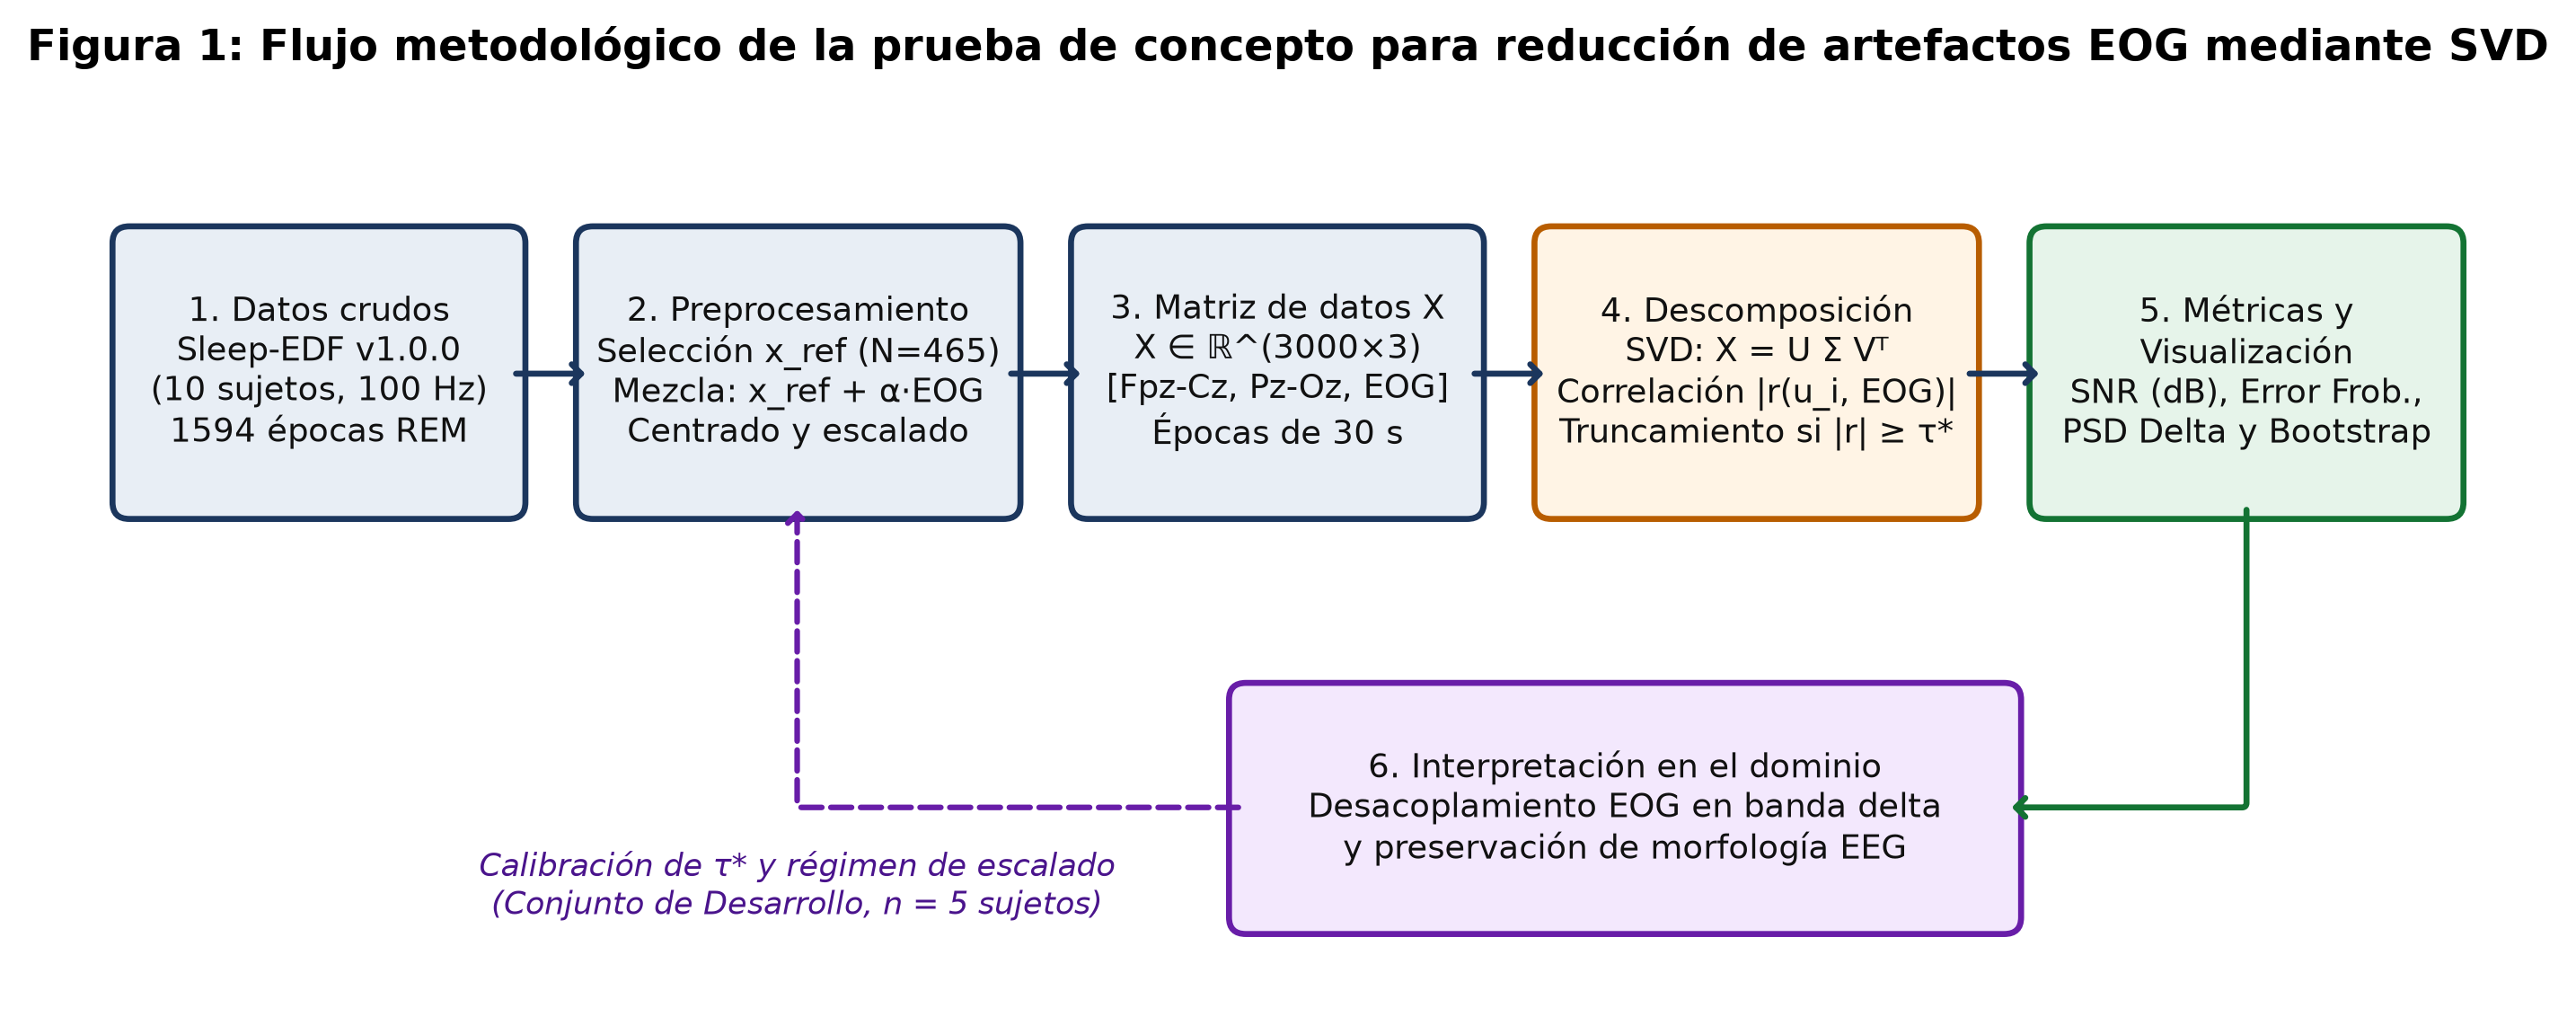
\includegraphics[width=\linewidth,height=4.05cm,keepaspectratio]{figures/fig1_flujo_metodologico.png}
      \end{tcolorbox}
      \vspace{0.04cm}
      \begin{tcolorbox}[navycard]
        \scriptsize\raggedright
        \textbf{Mezcla controlada basada en conducci\'on de volumen [2], [3]:}\\[0.04cm]
        $\bullet$ Canal Frontal: $x_{\text{cont, Fpz-Cz}}(t) = x_{\text{ref, Fpz-Cz}}(t) + \alpha \cdot eog(t)$\\
        $\bullet$ Canal Posterior: $x_{\text{cont, Pz-Oz}}(t) = x_{\text{ref, Pz-Oz}}(t) + 0.30\,\alpha \cdot eog(t)$\\
        evaluando 3 niveles de contaminaci\'on: $\alpha = 0.25$ (bajo), $0.50$ (moderado) y $0.80$ (severo).
      \end{tcolorbox}
    \end{column}

    \begin{column}{0.41\textwidth}
      \begin{tcolorbox}[basecard, title={\scriptsize\bfseries Partici\'on por Sujeto (\textit{Sleep-EDF v1.0.0} [1])}, colbacktitle=UDTeal!85!black, coltitle=white]
        \tiny
        \setlength{\tabcolsep}{2.8pt}
        \renewcommand{\arraystretch}{1.1}
        \begin{tabularx}{\linewidth}{@{}l Y r r r@{}}
          \toprule
          \textbf{Sujeto} & \textbf{Partici\'on} & \textbf{\'Ep. REM} & \textbf{$N_{\text{ref}}$} & \textbf{DE EOG ($\mu\text{V}$)} \\
          \midrule
          \texttt{SC4001} & Desarrollo & 125 & 35 & 41.3 \\
          \texttt{SC4011} & Desarrollo & 216 & 95 & 32.1 \\
          \texttt{SC4021} & Desarrollo & 192 & 50 & 31.8 \\
          \texttt{SC4031} & Desarrollo & 207 & 66 & 31.0 \\
          \texttt{SC4041} & Desarrollo & 123 & 36 & 42.6 \\
          \midrule
          \textbf{Subt. Dev} & \textbf{5 sujetos} & \textbf{863 ($431.5\text{ m}$)} & \textbf{282} & \textbf{35.8} \\
          \midrule
          \texttt{SC4051} & Evaluaci\'on & 84 & 16 & 39.2 \\
          \texttt{SC4061} & Evaluaci\'on & 133 & 40 & 29.8 \\
          \texttt{SC4071} & Evaluaci\'on & 198 & 49 & 36.4 \\
          \texttt{SC4081} & Evaluaci\'on & 141 & 41 & 38.9 \\
          \texttt{SC4091} & Evaluaci\'on & 175 & 37 & 35.1 \\
          \midrule
          \textbf{Subt. Eval} & \textbf{5 sujetos} & \textbf{731 ($365.5\text{ m}$)} & \textbf{183} & \textbf{35.9} \\
          \bottomrule
        \end{tabularx}
      \end{tcolorbox}
      \vspace{0.04cm}
      \begin{tcolorbox}[tealcard]
        \tiny
        \textbf{?`C\'omo se eligen las \'epocas limpias $x_{\text{ref}}$ ($N_{\text{total}}=465$)?}\\
        Se toman \'epocas REM tranquilas sin parpadeos ni sacadas ($|r(\text{EEG}, \text{EOG})| < 0.15$) y se combinan con los segmentos de mayor movimiento ocular del mismo paciente.
      \end{tcolorbox}
    \end{column}
  \end{columns}
\end{frame}

% ==============================================================================
% DIAPOSITIVA 7: PRUEBA DE CONCEPTO II - FORMULACION MATRICIAL SVD Y LINEA BASE
% ==============================================================================
\begin{frame}{La SVD descompone la \'epoca de 3 canales en 3 modos independientes y apaga el modo ocular}
  \framesubtitle{Secci\'on 3: Formulaci\'on matricial intuitiva, reg\'imenes de escalado y m\'etricas | Expositor: Cristian Aguilar}

  \begin{columns}[T,onlytextwidth]
    \begin{column}{0.52\textwidth}
      \begin{tcolorbox}[navycard, title={\scriptsize\bfseries ?`C\'omo funciona la SVD en cada \'epoca de 30 s? ($3000\text{ muestras}\times 3\text{ canales}$)}, colbacktitle=UDNavy, coltitle=white]
        \scriptsize
        \setlength{\abovedisplayskip}{3pt}\setlength{\belowdisplayskip}{3pt}
        Organizamos los 3 canales en una tabla $X$ de $3000\text{ filas}\times 3\text{ columnas}$ y la SVD la separa en la suma de \textbf{3 modos independientes}:
        \[
          X = \big[\, x_{\text{Fpz-Cz}} \;\;\; x_{\text{Pz-Oz}} \;\;\; x_{\text{EOG}} \,\big] = U \Sigma V^\top = \sigma_1 u_1 v_1^\top + \sigma_2 u_2 v_2^\top + \sigma_3 u_3 v_3^\top
        \]
        \begin{itemize}\scriptsize\setlength{\itemsep}{1pt}
          \item $u_i$ (\textbf{forma de onda en el tiempo}): patr\'on temporal de $3000$ puntos de cada modo.
          \item $\sigma_i$ (\textbf{amplitud o peso del modo}): ordenados de mayor a menor ($\sigma_1 \ge \sigma_2 \ge \sigma_3$). El porcentaje de energ\'ia de cada modo es $E_i = \sigma_i^2 / (\sigma_1^2 + \sigma_2^2 + \sigma_3^2)$ [7].
          \item $v_i$ (\textbf{peso en cada canal}): indica cu\'anto aparece ese modo en \texttt{Fpz-Cz}, \texttt{Pz-Oz} y \texttt{EOG}.
        \end{itemize}
      \end{tcolorbox}

      \vspace{0.04cm}

      \begin{tcolorbox}[tealcard, title={\scriptsize\bfseries Regla Sencilla de Limpieza (Truncamiento por Correlaci\'on)}, colbacktitle=UDTeal!85!black, coltitle=white]
        \scriptsize
        \begin{enumerate}\scriptsize\setlength{\itemsep}{1pt}
          \item Medimos la correlaci\'on $|r(u_i, \text{EOG})|$ de cada modo ($i=1,2,3$) con el canal ocular.
          \item Si $\mathbf{|r(u_i, \text{EOG})| \ge \tau^*}$ ($\tau^* = 0.50$), ese modo es el artefacto ocular $\to$ \textbf{lo apagamos haciendo $\sigma_i = 0$} y sumamos los modos restantes para obtener el EEG limpio $\widehat{X}$.
        \end{enumerate}
      \end{tcolorbox}
    \end{column}

    \begin{column}{0.46\textwidth}
      \begin{tcolorbox}[basecard, title={\scriptsize\bfseries Dos Formas de Preprocesar Antes de la SVD}, colbacktitle=UDNavy, coltitle=white]
        \scriptsize
        \textbf{1. R\'egimen A (\texttt{SVD\_Fisico\_uV}): Escala f\'isica en microvoltios ($\mu\text{V}$)}\\
        Solo resta el promedio de cada canal. Conserva el tama\~no natural de las se\~nales: el ojo ($\approx 39.7\,\mu\text{V}$) es casi $4$ veces m\'as grande que el EEG ($\approx 10.0\,\mu\text{V}$) [8].\\[0.08cm]
        \textbf{2. R\'egimen B (\texttt{SVD\_Zscore}): Normalizaci\'on Z-score por canal}\\
        Divide cada canal por su desviaci\'on est\'andar para forzar a que los 3 canales tengan varianza igual a $1$ antes de aplicar la SVD.
      \end{tcolorbox}

      \vspace{0.04cm}

      \begin{tcolorbox}[ambercard, title={\scriptsize\bfseries Comparadores y M\'etricas de Evaluaci\'on}, colbacktitle=UDAmber!85!black, coltitle=white]
        \scriptsize
        \begin{itemize}\setlength{\itemsep}{1pt}
          \item \textbf{Comparadores:} Se\~nal contaminada sin procesar (\texttt{Raw}) y filtro pasa-banda \textbf{Butterworth} ($0.5\text{--}30\text{ Hz}$).
          \item \textbf{Relaci\'on Se\~nal a Ruido ($\text{SNR}$ en dB):}
            $\text{SNR} = 10\log_{10}\!\left(\text{Energ\'ia de } x_{\text{ref}} \,/\, \text{Energ\'ia del error}\right)$ (m\'as alta es mejor).
          \item \textbf{Errores ($\varepsilon_{\text{Frob}}$ y $\varepsilon_{\text{PSD},\delta}$):} miden el error total de la onda y el error en banda delta $0.5\text{--}4\text{ Hz}$ (m\'as cercanos a $0$ es mejor).
        \end{itemize}
      \end{tcolorbox}
    \end{column}
  \end{columns}
\end{frame}

% ==============================================================================
% DIAPOSITIVA 8: RESULTADOS CUANTITATIVOS I - CALIBRACION DEL UMBRAL EN DESARROLLO
% ==============================================================================
\begin{frame}{El barrido en desarrollo identifica un umbral \'optimo $\tau^* = 0.50$ con una meseta estable en escala f\'isica}
  \framesubtitle{Secci\'on 4: Resultados cuantitativos I (Calibraci\'on en Desarrollo, $N_{\text{dev}}=282$ \'epocas) | Expositor: Cristian Aguilar}

  \begin{columns}[T,onlytextwidth]
    \begin{column}{0.56\textwidth}
      \begin{tcolorbox}[basecard, title={\scriptsize\bfseries Curva de Sensibilidad del Umbral $\tau$ (Figura 3)}, colbacktitle=UDNavy, coltitle=white]
        \centering
        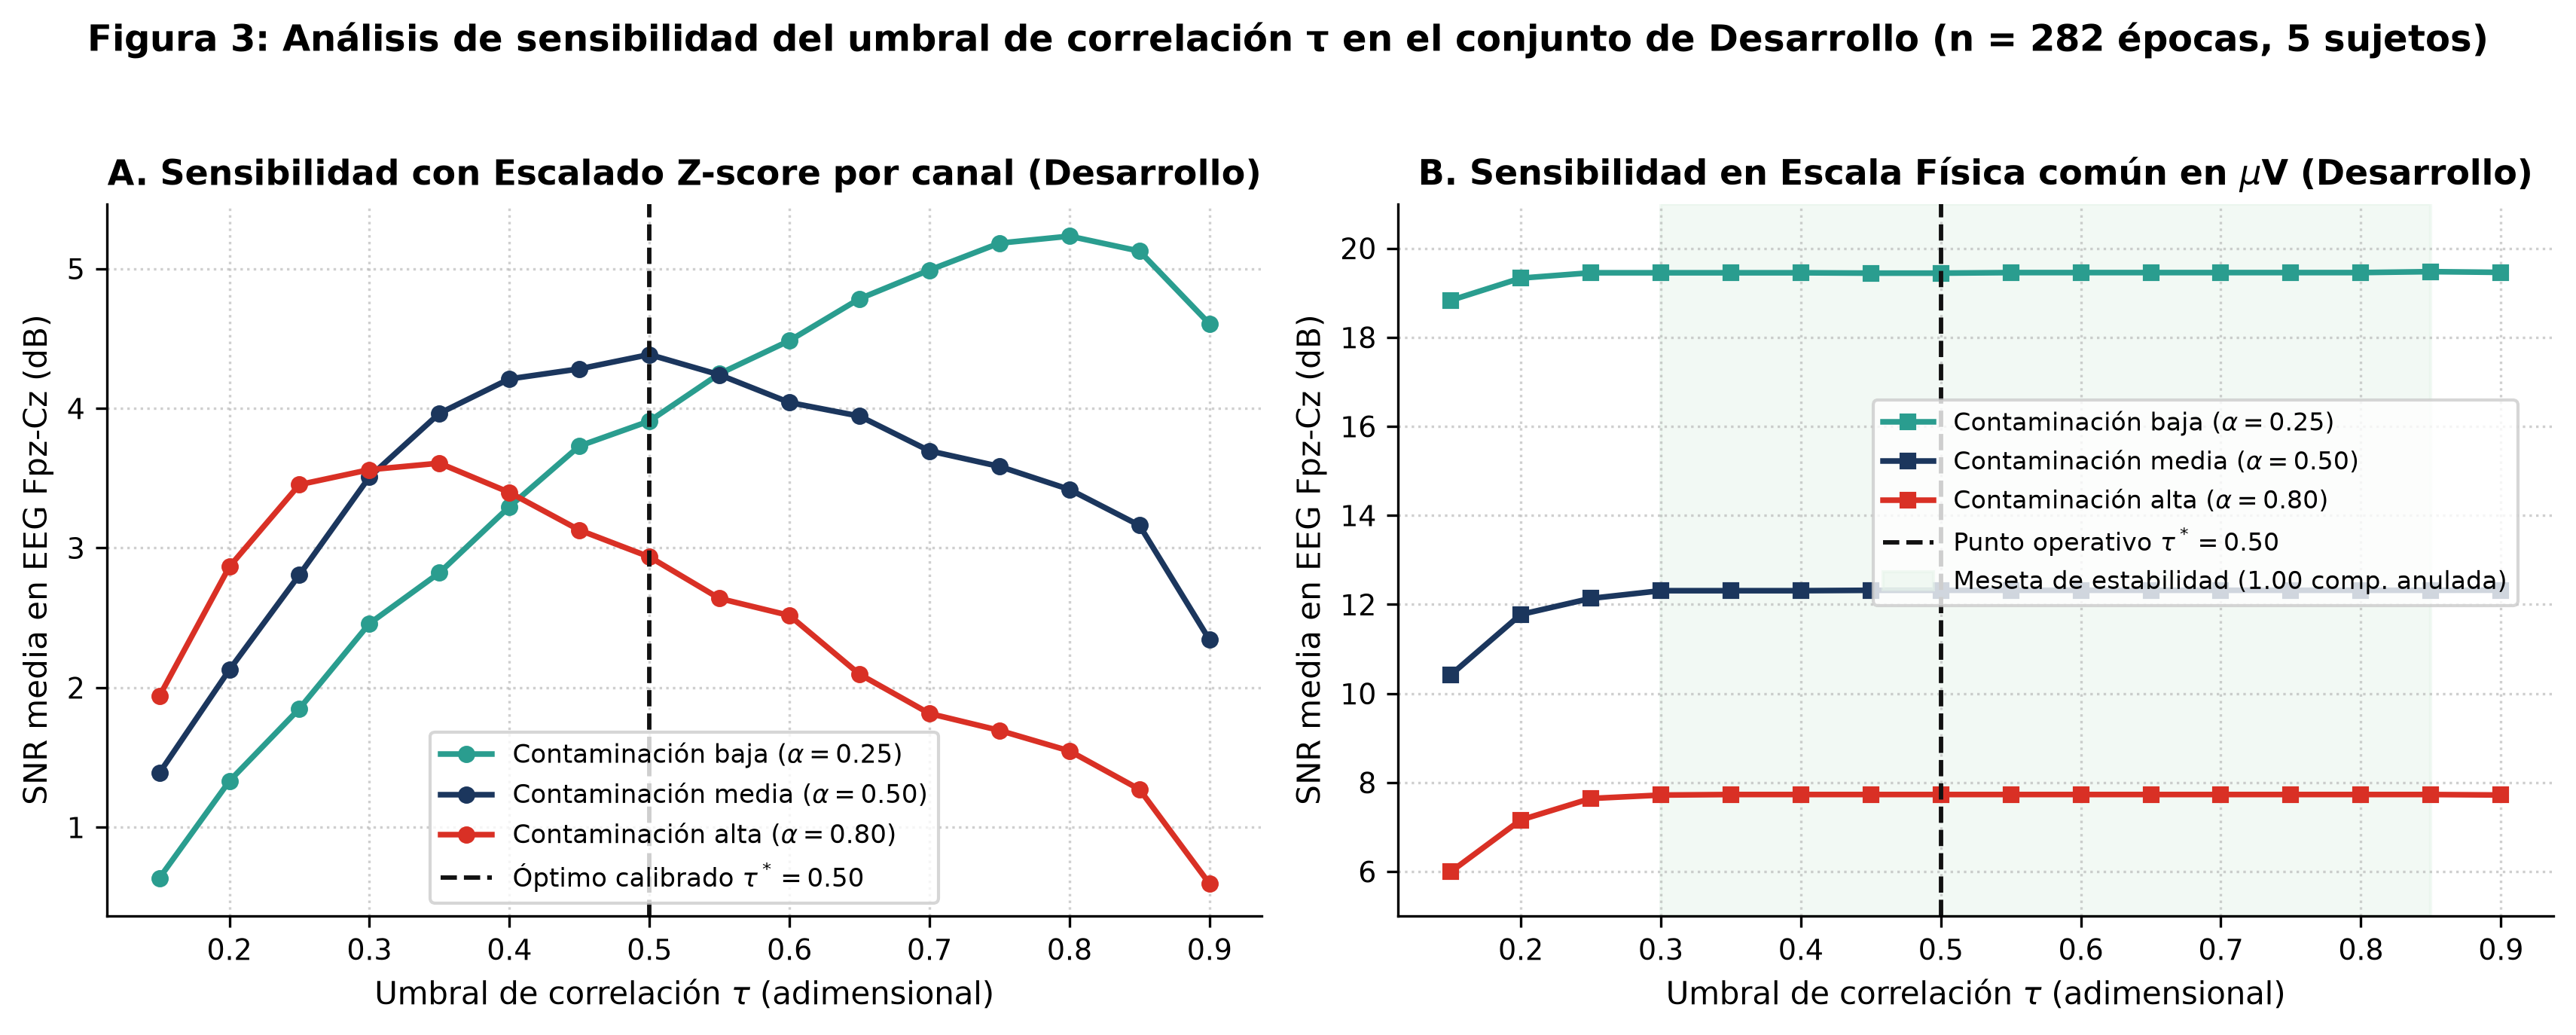
\includegraphics[width=\linewidth,height=4.85cm,keepaspectratio]{figures/fig3_sensibilidad_umbral_desarrollo.png}
      \end{tcolorbox}
    \end{column}

    \begin{column}{0.42\textwidth}
      \begin{tcolorbox}[basecard, title={\scriptsize\bfseries Barrido de $\tau$ en Desarrollo ($\alpha=0.50, N_{\text{dev}}=282$)}, colbacktitle=UDTeal!85!black, coltitle=white]
        \tiny
        \setlength{\tabcolsep}{2.5pt}
        \renewcommand{\arraystretch}{1.1}
        \begin{tabularx}{\linewidth}{@{}Y r r r r@{}}
          \toprule
          \textbf{Umbral $\tau$} & \textbf{SNR ($\mu\text{V}$)} & \textbf{Comp. ($\mu\text{V}$)} & \textbf{SNR (Z)} & \textbf{Comp. (Z)} \\
          \midrule
          $0.20$ & $+10.76\text{ dB}$ & $1.13$ & $+3.95\text{ dB}$ & $1.97$ \\
          $0.30$ & $+10.89\text{ dB}$ & $1.01$ & $+4.44\text{ dB}$ & $1.86$ \\
          $0.40$ & $+10.89\text{ dB}$ & $1.01$ & $+5.22\text{ dB}$ & $1.62$ \\
          \textbf{0.50 ($\tau^*$)} & $\mathbf{+10.89\text{ dB}}$ & $\mathbf{1.01}$ & $\mathbf{+5.90\text{ dB}}$ & $\mathbf{1.27}$ \\
          $0.60$ & $+10.89\text{ dB}$ & $1.01$ & $+5.36\text{ dB}$ & $0.96$ \\
          $0.70$ & $+10.89\text{ dB}$ & $1.01$ & $+3.07\text{ dB}$ & $0.76$ \\
          $0.80$ & $+10.86\text{ dB}$ & $1.00$ & $+0.24\text{ dB}$ & $0.36$ \\
          \bottomrule
        \end{tabularx}
      \end{tcolorbox}

      \vspace{0.08cm}

      \begin{tcolorbox}[tealcard, title={\scriptsize\bfseries ?`Por qu\'e elegimos $\tau^* = 0.50$?}, colbacktitle=UDTeal!85!black, coltitle=white]
        \scriptsize
        \begin{itemize}
          \item \textbf{Estabilidad total en escala f\'isica ($\mu\text{V}$):} Entre $\tau=0.25$ y $\tau=0.70$, la $\text{SNR}$ en \texttt{Fpz-Cz} se mantiene fija en $+10.89\text{ dB}$, apagando siempre el Modo 1 ($1.01$ modos en promedio).
          \item \textbf{Mejor punto para Z-score:} En $\tau^*=0.50$ el m\'etodo Z-score logra su punto m\'as alto ($+5.90\text{ dB}$).
          \item \textbf{Sin trampa experimental:} Fijamos $\tau^*=0.50$ usando solo los 5 sujetos de Desarrollo antes de evaluar los 5 sujetos de prueba.
        \end{itemize}
      \end{tcolorbox}
    \end{column}
  \end{columns}
\end{frame}

% ==============================================================================
% DIAPOSITIVA 9: RESULTADOS CUANTITATIVOS II - ESPECTRO SVD EN EVALUACION
% ==============================================================================
\begin{frame}{El primer modo singular concentra entre 82.3\% y 90.3\% de la energ\'ia con correlaci\'on EOG de 0.98}
  \framesubtitle{Secci\'on 4: Resultados cuantitativos II (Energ\'ia y correlaci\'on en Evaluaci\'on, $N_{\text{eval}}=183$ \'epocas) | Expositor: Sergio Osorio}

  \begin{columns}[T,onlytextwidth]
    \begin{column}{0.54\textwidth}
      \begin{tcolorbox}[basecard, title={\scriptsize\bfseries Distribuci\'on de Energ\'ia y Correlaci\'on EOG (Figura 2)}, colbacktitle=UDNavy, coltitle=white]
        \centering
        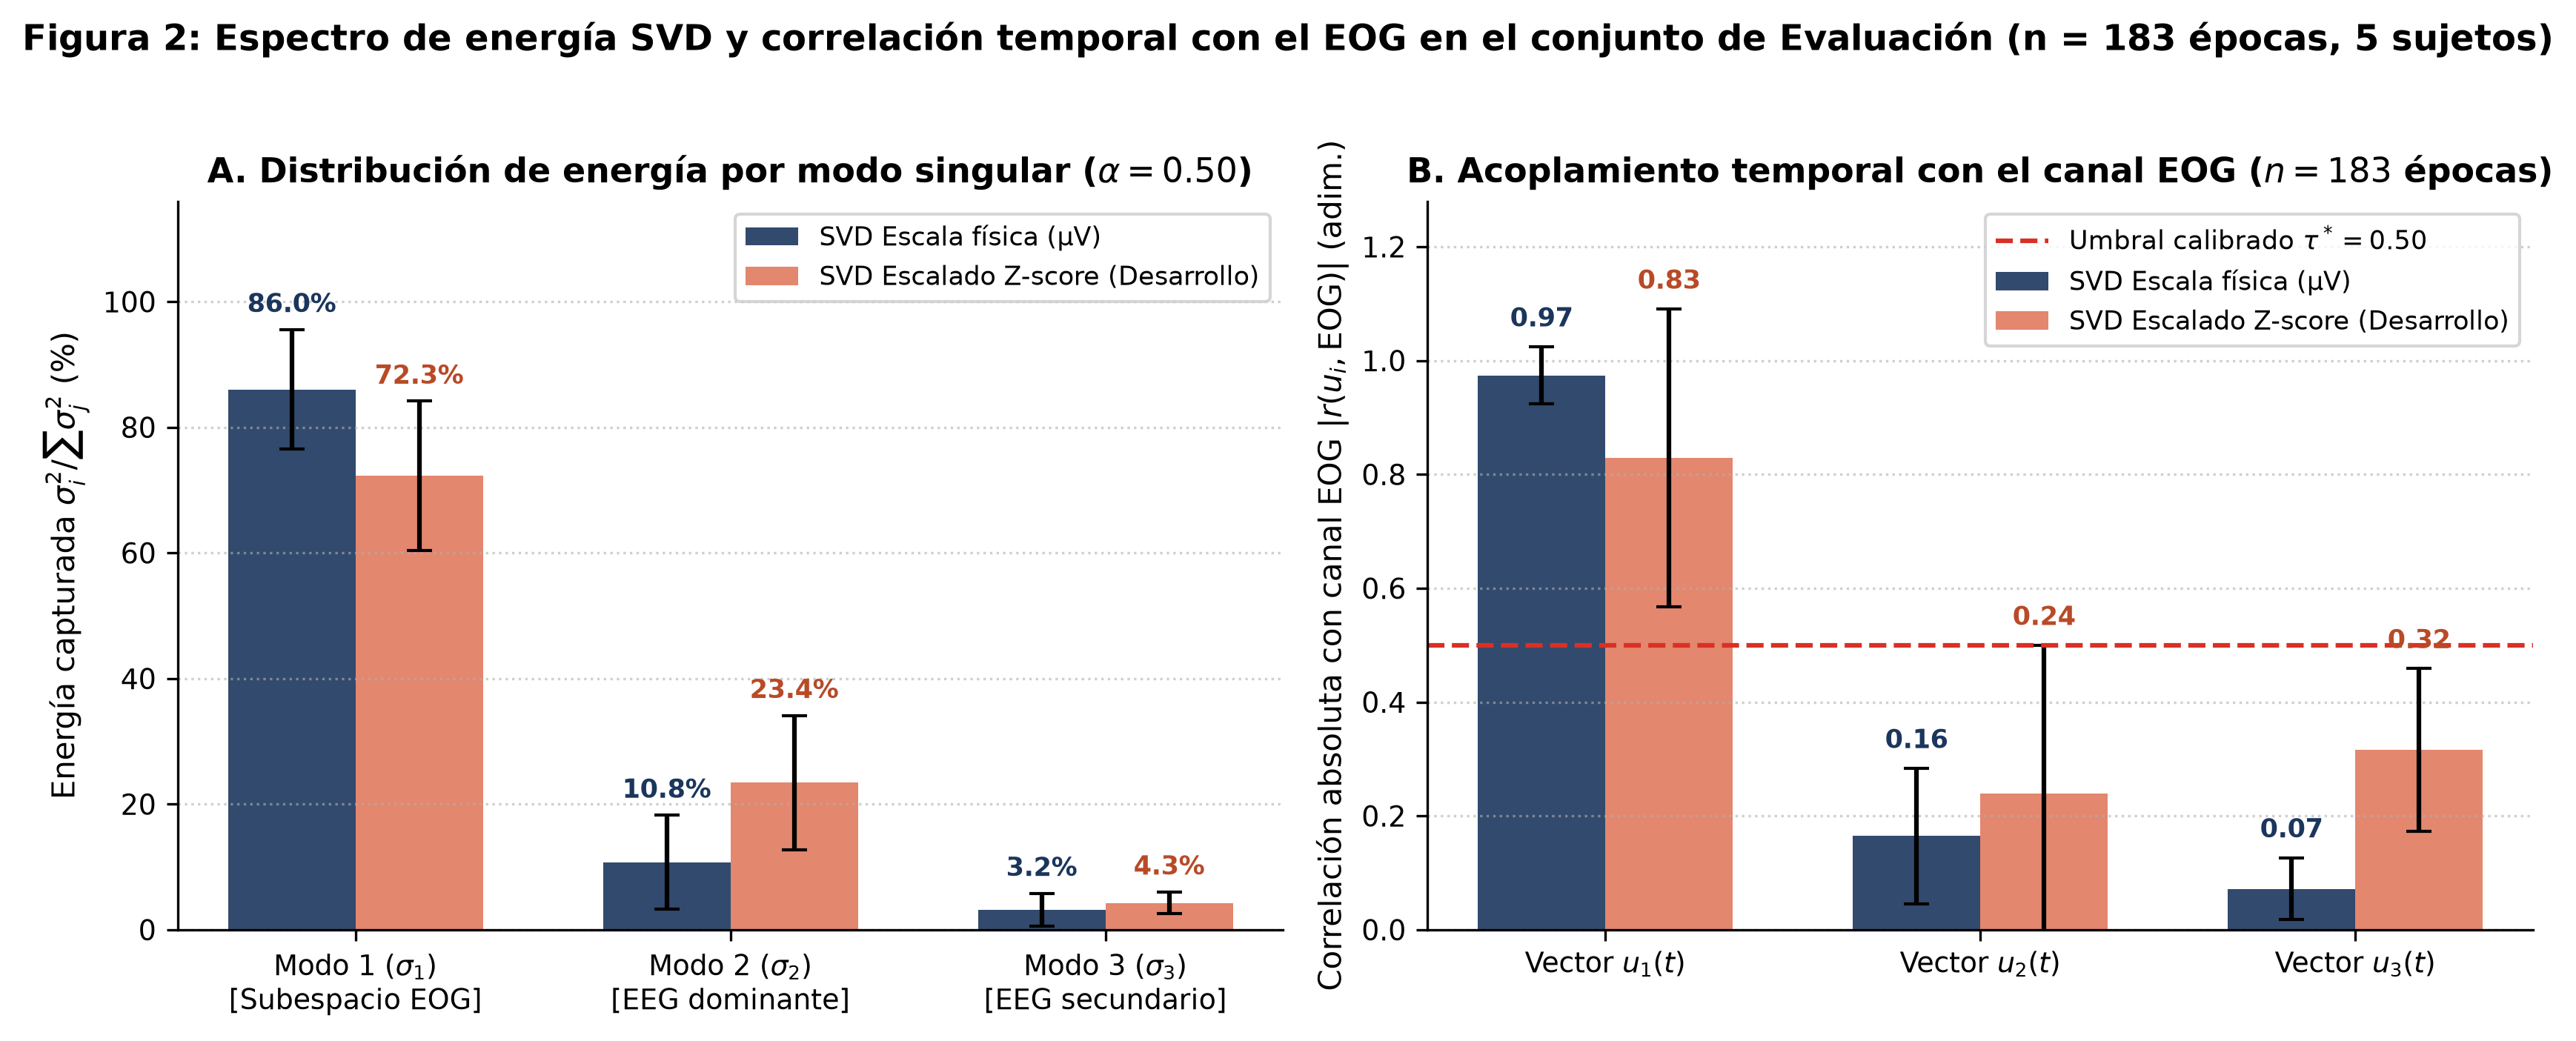
\includegraphics[width=\linewidth,height=4.85cm,keepaspectratio]{figures/fig2_espectro_svd_y_correlacion.png}
      \end{tcolorbox}
    \end{column}

    \begin{column}{0.44\textwidth}
      \begin{tcolorbox}[basecard, title={\scriptsize\bfseries Energ\'ia por Modo en Evaluaci\'on ($N_{\text{eval}}=183$, Media $\pm$ DE)}, colbacktitle=UDNavy, coltitle=white]
        \tiny
        \setlength{\tabcolsep}{2.2pt}
        \renewcommand{\arraystretch}{1.1}
        \begin{tabularx}{\linewidth}{@{}Y c r r r@{}}
          \toprule
          \textbf{R\'egimen} & $\boldsymbol{\alpha}$ & \textbf{$E_1 / E_2 / E_3$ (\%)} & $\boldsymbol{|r(u_1,\text{EOG})|}$ & $\boldsymbol{|r(u_2,\text{EOG})|}$ \\
          \midrule
          \texttt{F\'isico ($\mu\text{V}$)} & $0.25$ & $\mathbf{82.3} / 11.5 / 6.3$ & $\mathbf{0.97 \pm 0.13}$ & $0.13 \pm 0.12$ \\
          \texttt{F\'isico ($\mu\text{V}$)} & $0.50$ & $\mathbf{86.0} / 9.0 / 4.9$ & $\mathbf{0.98 \pm 0.11}$ & $0.16 \pm 0.11$ \\
          \texttt{F\'isico ($\mu\text{V}$)} & $0.80$ & $\mathbf{90.3} / 6.3 / 3.4$ & $\mathbf{0.98 \pm 0.10}$ & $0.17 \pm 0.10$ \\
          \midrule
          \texttt{Z-score} & $0.25$ & $48.7 / 30.9 / 20.4$ & $0.66 \pm 0.34$ & $0.41 \pm 0.29$ \\
          \texttt{Z-score} & $0.50$ & $60.8 / 23.0 / 16.3$ & $0.86 \pm 0.21$ & $0.32 \pm 0.19$ \\
          \texttt{Z-score} & $0.80$ & $74.9 / 14.5 / 10.6$ & $0.95 \pm 0.13$ & $0.24 \pm 0.12$ \\
          \bottomrule
        \end{tabularx}
      \end{tcolorbox}

      \vspace{0.08cm}

      \begin{tcolorbox}[navycard, title={\scriptsize\bfseries ?`Qu\'e nos dicen estos n\'umeros?}, colbacktitle=UDNavy, coltitle=white]
        \scriptsize
        \begin{itemize}
          \item \textbf{En escala f\'isica ($\mu\text{V}$) el ojo queda atrapado en el Modo 1:} En los tres niveles de contaminaci\'on, el Modo 1 concentra m\'as del $82\%$ de la energ\'ia total y tiene una correlaci\'on de $0.97\text{ a }0.98$ con el canal EOG, mientras que los Modos 2 y 3 tienen correlaci\'on muy baja ($\le 0.17$) y guardan el EEG limpio.
          \item \textbf{En Z-score con bajo artefacto ($\alpha=0.25$) el ojo se reparte:} La energ\'ia se divide ($48.7\%$ y $30.9\%$) y el parpadeo/sacada se mezcla en los tres modos ($|r|=0.66, 0.41, 0.45$).
        \end{itemize}
      \end{tcolorbox}
    \end{column}
  \end{columns}
\end{frame}

% ==============================================================================
% DIAPOSITIVA 10: RESULTADOS CUANTITATIVOS III - SNR, FROBENIUS Y BOOTSTRAP
% ==============================================================================
\begin{frame}{La SVD en escala f\'isica logra ganancias de +13.9 a +14.9 dB y verifica la hip\'otesis con IC 95\% > 0}
  \framesubtitle{Secci\'on 4: Resultados cuantitativos III (Desempe\~no en Evaluaci\'on e intervalos de confianza, $N_{\text{eval}}=183$) | Expositor: Sergio Osorio}

  \begin{columns}[T,onlytextwidth]
    \begin{column}{0.49\textwidth}
      \begin{tcolorbox}[basecard, title={\scriptsize\bfseries Comparaci\'on de SNR e Intervalos Bootstrap (Figura 4)}, colbacktitle=UDNavy, coltitle=white]
        \centering
        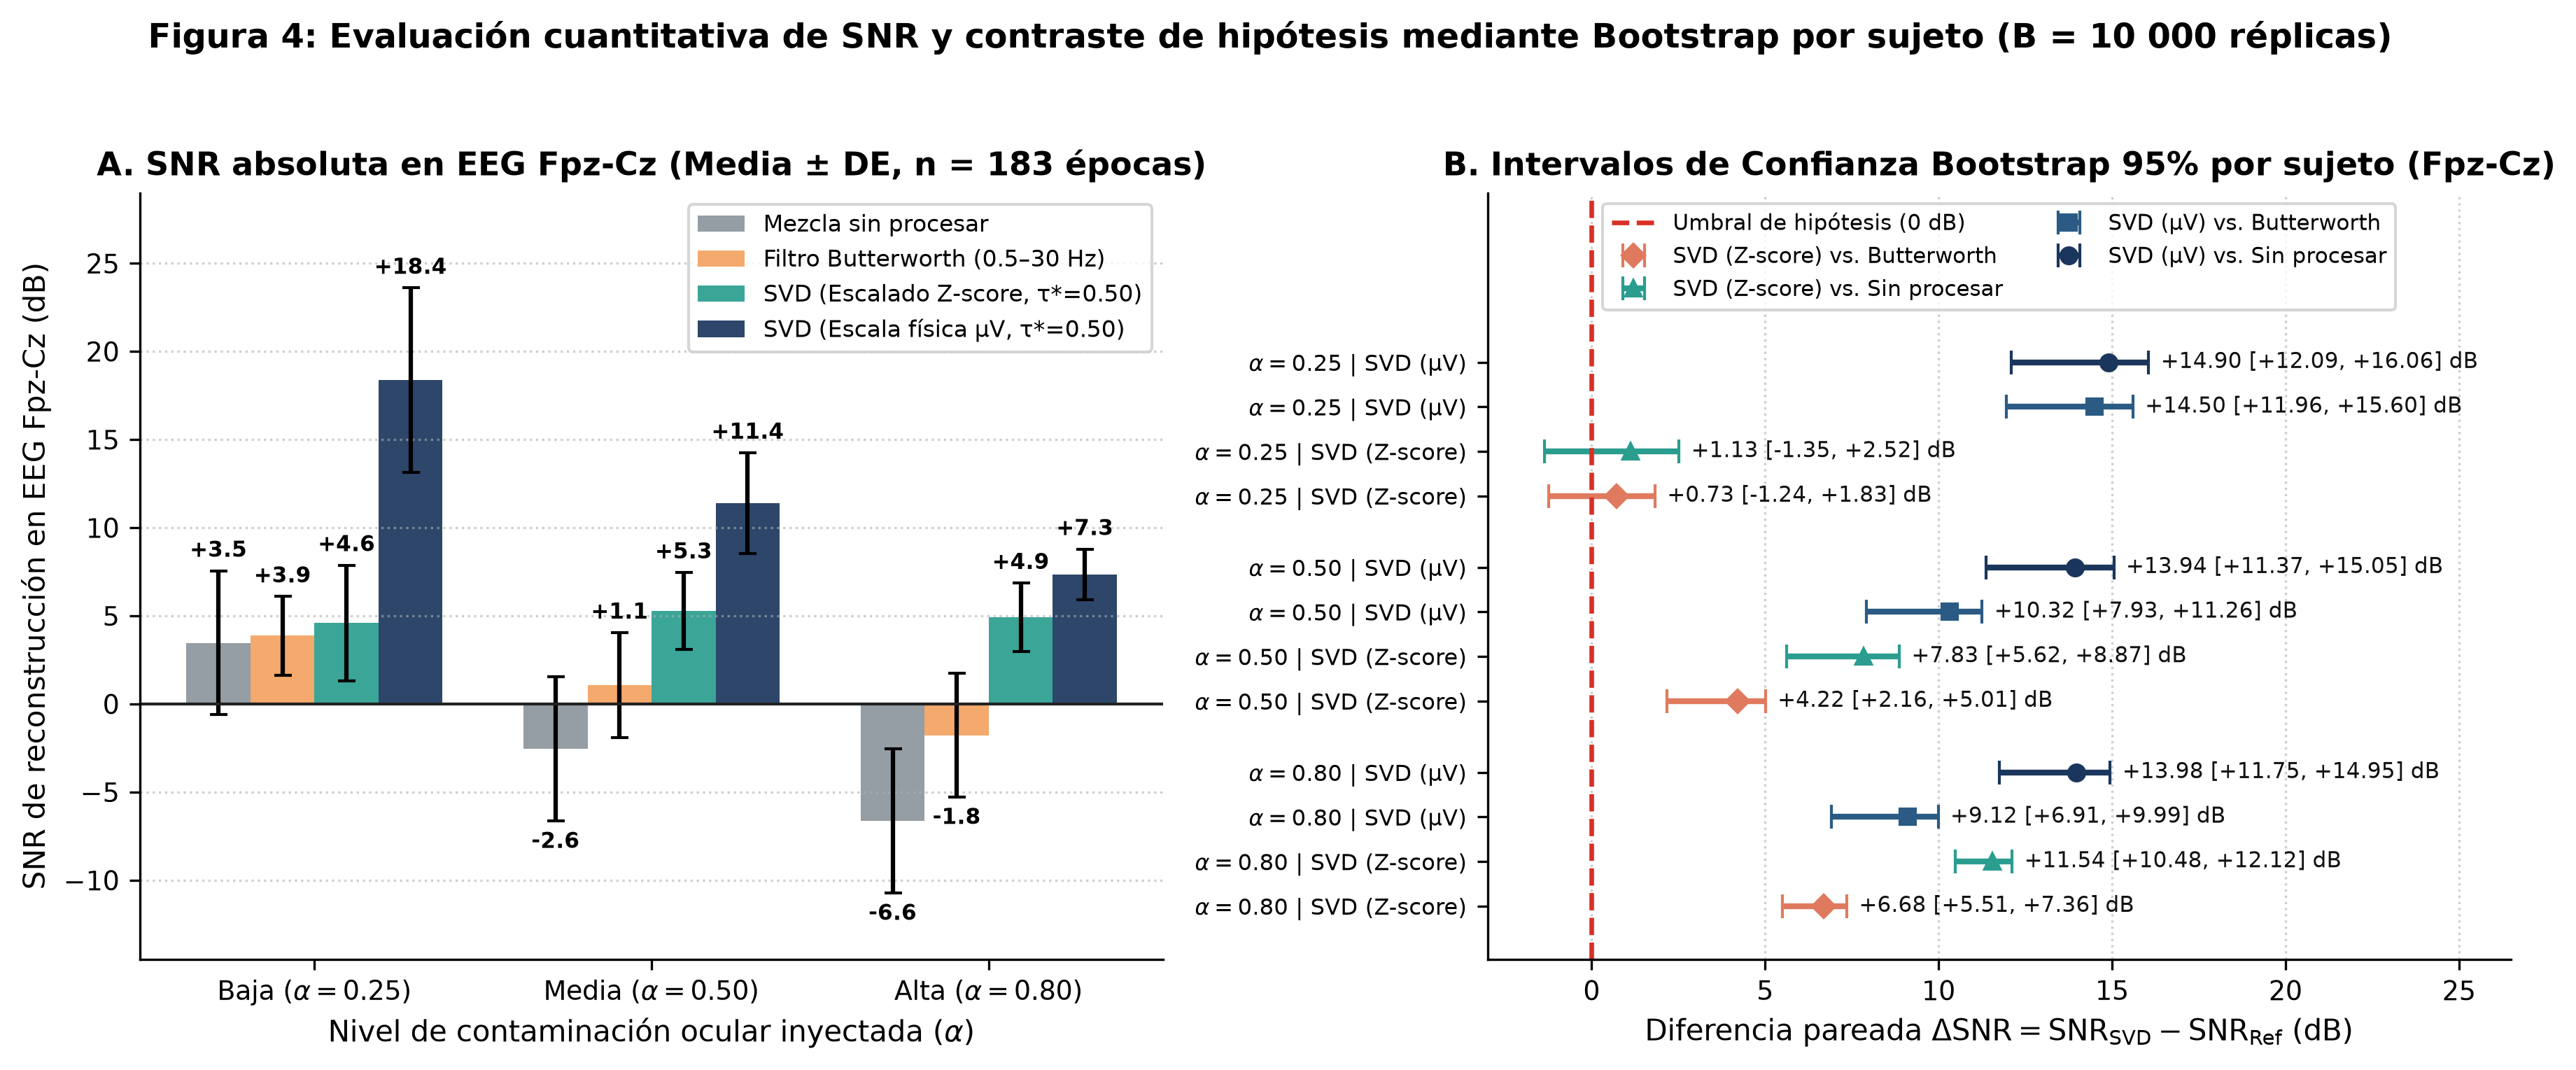
\includegraphics[width=\linewidth,height=4.85cm,keepaspectratio]{figures/fig4_comparacion_snr_bootstrap.png}
      \end{tcolorbox}
    \end{column}

    \begin{column}{0.49\textwidth}
      \begin{tcolorbox}[basecard, title={\scriptsize\bfseries Desempe\~no en Canal Frontal \texttt{Fpz-Cz} ($N_{\text{eval}}=183$ \'epocas)}, colbacktitle=UDTeal!85!black, coltitle=white]
        \tiny
        \setlength{\tabcolsep}{2.2pt}
        \renewcommand{\arraystretch}{1.06}
        \begin{tabularx}{\linewidth}{@{}Y c r r r r@{}}
          \toprule
          \textbf{M\'etodo} & $\boldsymbol{\alpha}$ & \textbf{SNR (dB)} & $\boldsymbol{\varepsilon_{\text{Frob}}}$ & $\boldsymbol{\varepsilon_{\text{PSD},\delta}}$ & \textbf{$\Delta\text{SNR}_{\text{vs Butt}}$ [IC 95\% suj.]} \\
          \midrule
          \texttt{Sin procesar} & $0.25$ & $+3.47$ & $0.652$ & $0.440$ & $-0.41\text{ dB}$ \\
          \texttt{Butterworth} & $0.25$ & $+3.87$ & $0.630$ & $0.517$ & Referencia ($0.00\text{ dB}$) \\
          \textbf{\texttt{SVD ($\mu\text{V}$)}} & $\mathbf{0.25}$ & $\mathbf{+18.37}$ & $\mathbf{0.123}$ & $\mathbf{0.193}$ & $\mathbf{+14.50\text{ dB}\;[+11.96, +15.60]}$ \\
          \texttt{SVD (Z-score)} & $0.25$ & $+4.60$ & $0.684$ & $0.655$ & $+0.73\text{ dB}\;[-1.63, +2.07]$ \\
          \midrule
          \texttt{Sin procesar} & $0.50$ & $-2.55$ & $1.305$ & $1.760$ & $-3.62\text{ dB}$ \\
          \texttt{Butterworth} & $0.50$ & $+1.07$ & $0.867$ & $1.263$ & Referencia ($0.00\text{ dB}$) \\
          \textbf{\texttt{SVD ($\mu\text{V}$)}} & $\mathbf{0.50}$ & $\mathbf{+11.39}$ & $\mathbf{0.257}$ & $\mathbf{0.419}$ & $\mathbf{+10.32\text{ dB}\;[+7.93, +11.26]}$ \\
          \texttt{SVD (Z-score)} & $0.50$ & $+5.28$ & $0.579$ & $0.692$ & $+4.22\text{ dB}\;[+2.16, +5.01]$ \\
          \midrule
          \texttt{Sin procesar} & $0.80$ & $-6.63$ & $2.088$ & $4.506$ & $-4.87\text{ dB}$ \\
          \texttt{Butterworth} & $0.80$ & $-1.77$ & $1.186$ & $2.927$ & Referencia ($0.00\text{ dB}$) \\
          \textbf{\texttt{SVD ($\mu\text{V}$)}} & $\mathbf{0.80}$ & $\mathbf{+7.35}$ & $\mathbf{0.415}$ & $\mathbf{0.556}$ & $\mathbf{+9.12\text{ dB}\;[+6.91, +9.99]}$ \\
          \texttt{SVD (Z-score)} & $0.80$ & $+4.91$ & $0.592$ & $0.761$ & $+6.68\text{ dB}\;[+5.51, +7.36]$ \\
          \bottomrule
        \end{tabularx}
      \end{tcolorbox}

      \vspace{0.06cm}

      \begin{tcolorbox}[tealcard, title={\scriptsize\bfseries Verificaci\'on de la Hip\'otesis de Investigaci\'on}, colbacktitle=UDTeal!85!black, coltitle=white]
        \tiny
        \begin{itemize}
          \item \textbf{\texttt{SVD\_Fisico\_uV} cumple la hip\'otesis en todos los casos:} Sus intervalos de confianza al $95\%$ están completamente a la derecha de la l\'inea roja ($0\text{ dB}$), superando a la se\~nal cruda en $+13.9\text{ a }+14.9\text{ dB}$ y a Butterworth en $+9.1\text{ a }+14.5\text{ dB}$.
          \item \textbf{Recuperaci\'on de banda delta:} En $\alpha=0.50$, baja el error espectral delta de $1.760$ (cruda) y $1.263$ (Butterworth) a $\mathbf{0.419}$ ($66.8\%$ menos error que Butterworth).
        \end{itemize}
      \end{tcolorbox}
    \end{column}
  \end{columns}
\end{frame}

% ==============================================================================
% DIAPOSITIVA 11: RESULTADOS CUALITATIVOS I Y II - VECTORES SINGULARES Y PSD
% ==============================================================================
\begin{frame}{El modo dominante captura la morfolog\'ia ocular en baja frecuencia y restaura la banda delta frontal}
  \framesubtitle{Secci\'on 4: Resultados cualitativos I y II (Interpretaci\'on visual de los modos y reconstrucci\'on de la onda) | Expositor: Nicolas Velasco}

  \begin{columns}[T,onlytextwidth]
    \begin{column}{0.49\textwidth}
      \begin{tcolorbox}[basecard, title={\scriptsize\bfseries Modos Temporales $\sigma_i u_i(t)$ y Nube de Puntos (Figura 5)}, colbacktitle=UDNavy, coltitle=white]
        \centering
        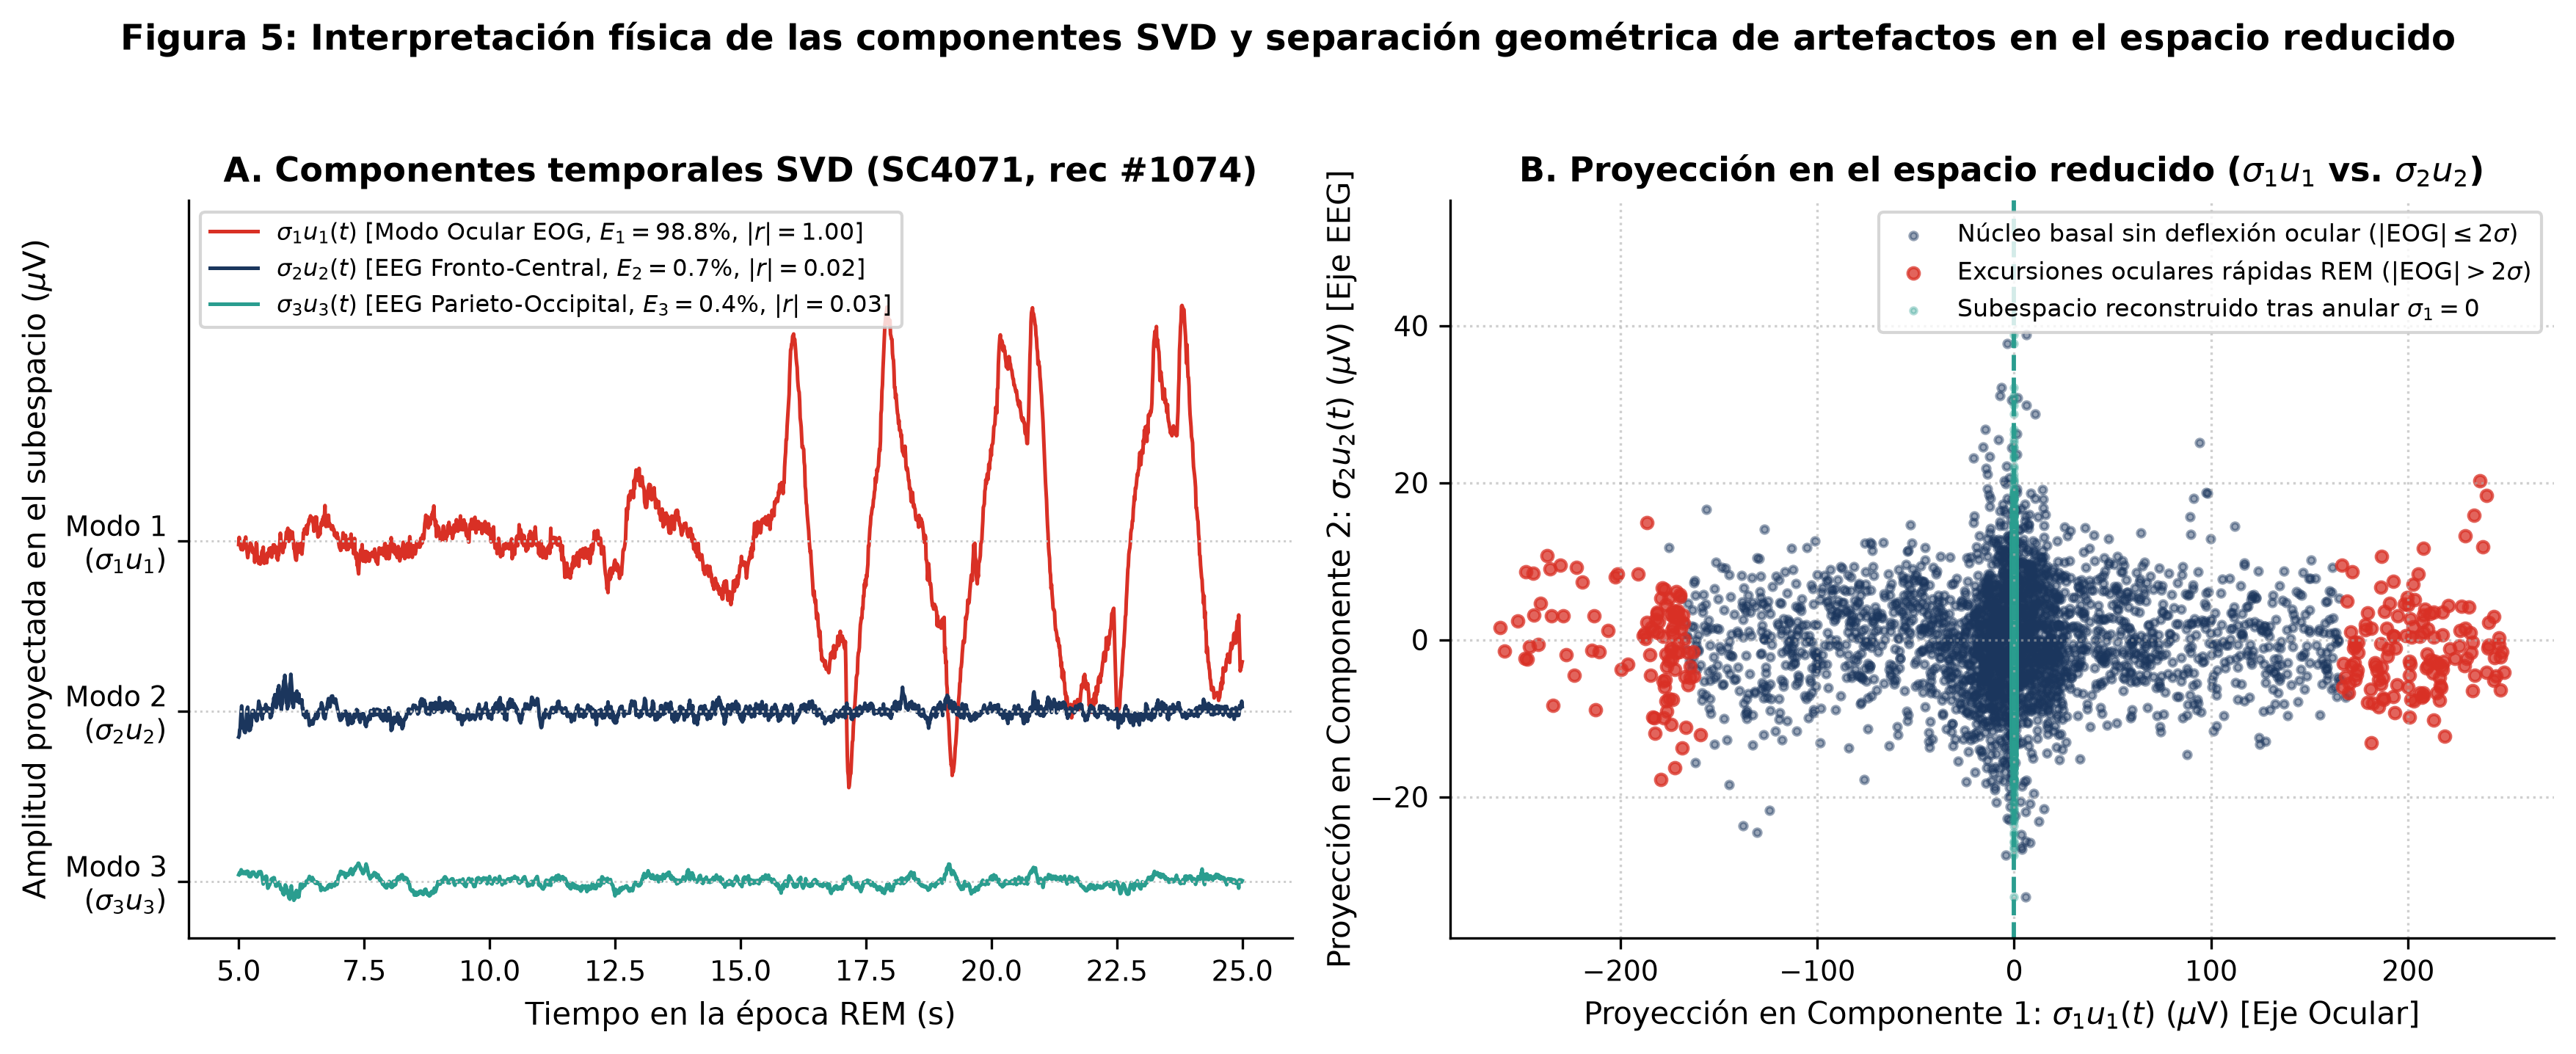
\includegraphics[width=\linewidth,height=3.95cm,keepaspectratio]{figures/fig5_vectores_singulares_y_subespacio.png}
      \end{tcolorbox}
      \vspace{0.04cm}
      \begin{tcolorbox}[navycard]
        \tiny
        \textbf{?`Qu\'e representa cada modo en la pr\'actica? (\texttt{SC4071}, $\alpha=0.50$):}
        \begin{itemize}\tiny
          \item El \textbf{Modo 1} (rojo) copia exactamente las sacadas grandes del ojo ($|r| = 1.00$, $E_1 = 98.8\%$).
          \item Los \textbf{Modos 2 y 3} (azul y verde) contienen las oscilaciones r\'apidas del cerebro sin rastro de parpadeos ($|r| \le 0.03$).
        \end{itemize}
      \end{tcolorbox}
    \end{column}

    \begin{column}{0.49\textwidth}
      \begin{tcolorbox}[basecard, title={\scriptsize\bfseries Reconstrucci\'on en el Tiempo y Frecuencia (Figura 6)}, colbacktitle=UDTeal!85!black, coltitle=white]
        \centering
        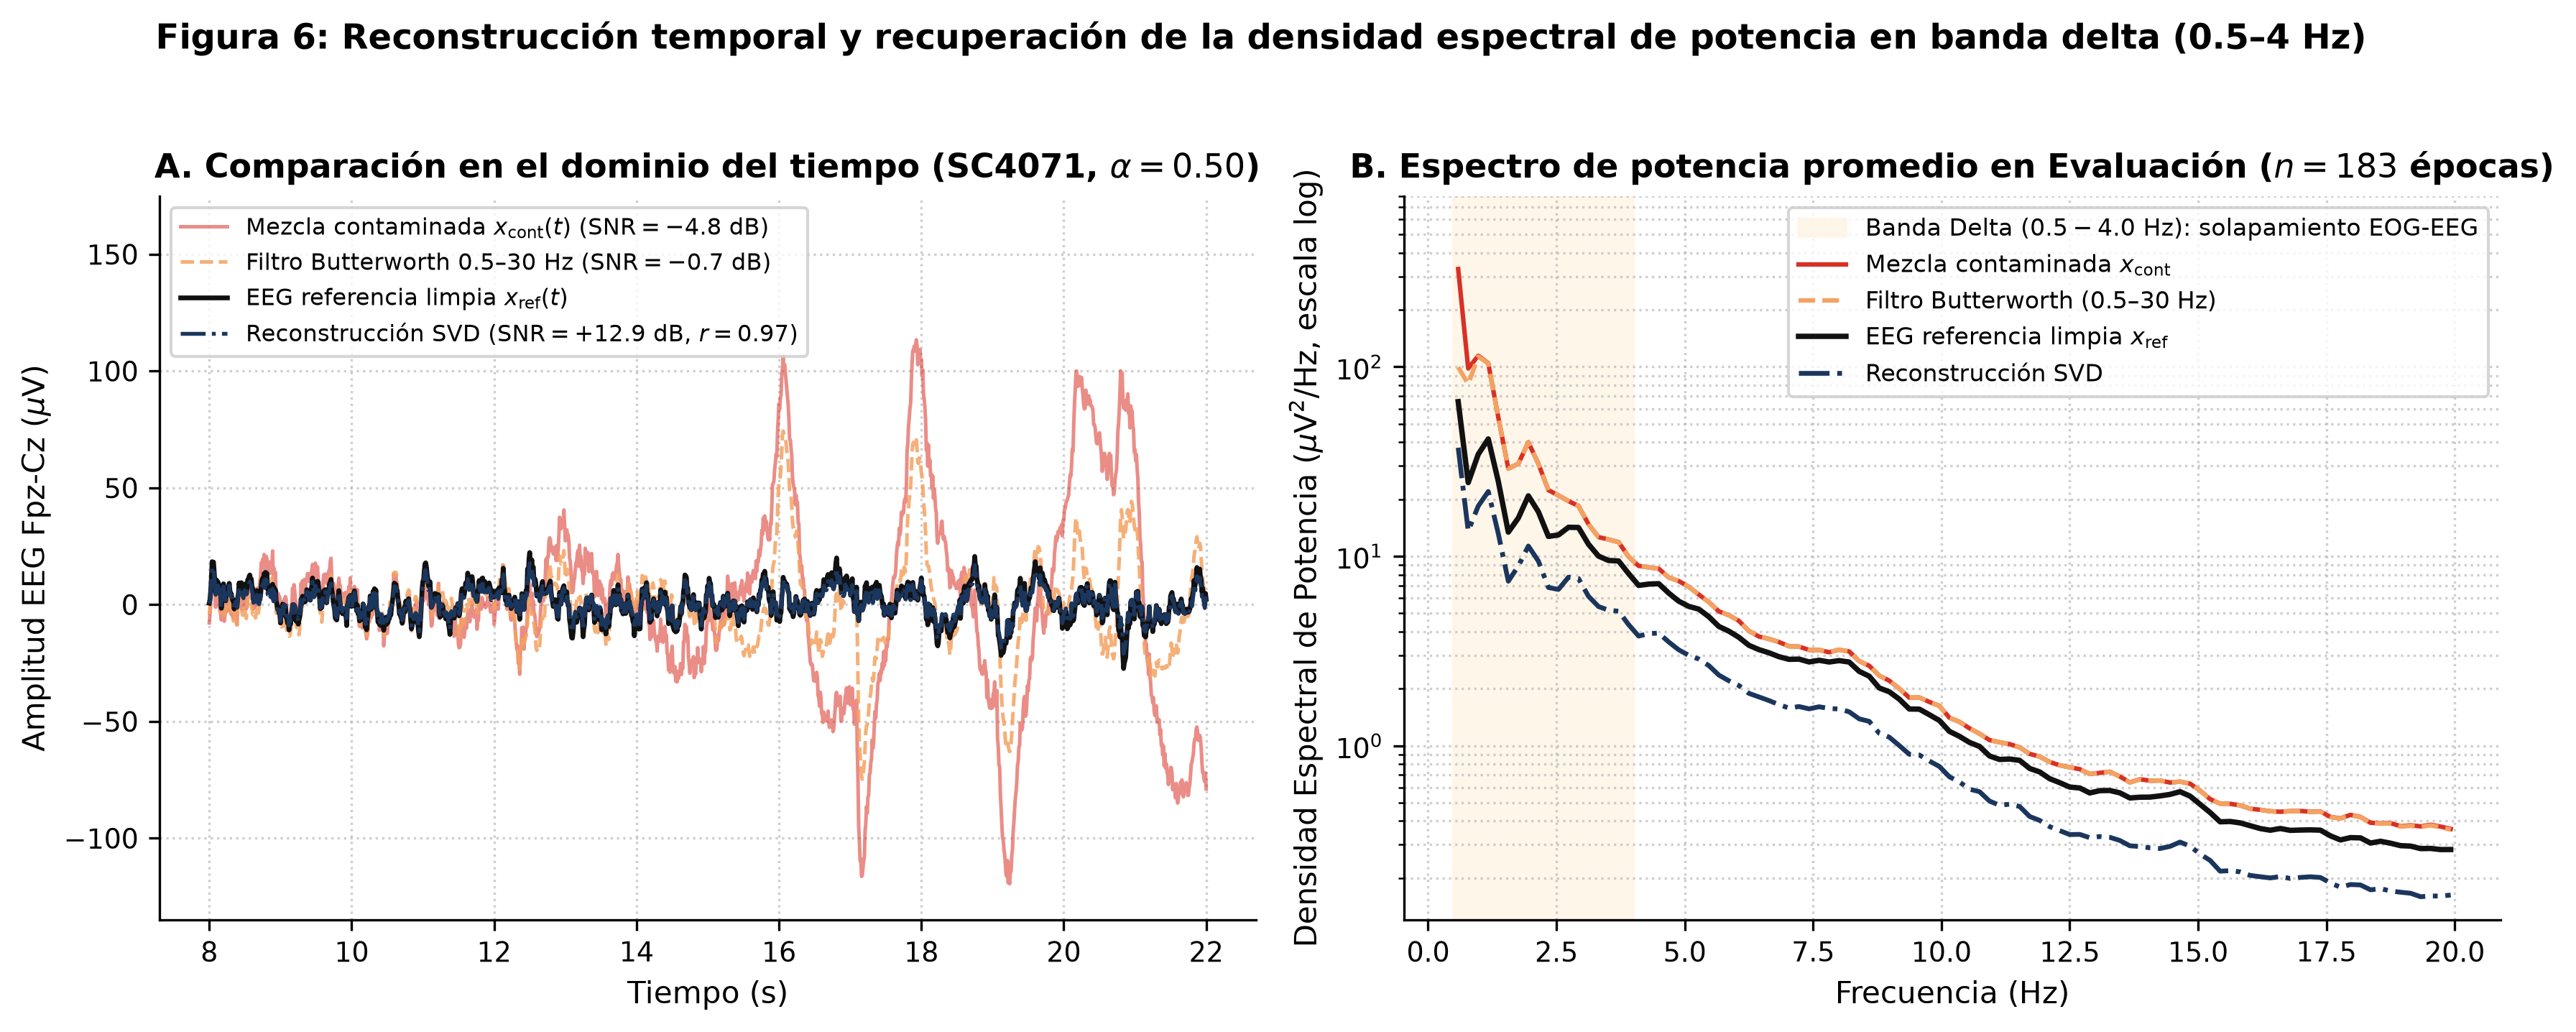
\includegraphics[width=\linewidth,height=3.95cm,keepaspectratio]{figures/fig6_reconstruccion_temporal_y_psd.png}
      \end{tcolorbox}
      \vspace{0.04cm}
      \begin{tcolorbox}[tealcard]
        \tiny
        \textbf{Comparaci\'on visual frente al filtro Butterworth:}
        \begin{itemize}\tiny
          \item Cuando el ojo se mueve fuerte ($t \in [14, 21]\text{ s}$), Butterworth (l\'inea naranja) se deforma igual que la se\~nal contaminada ($\text{SNR}=-0.7\text{ dB}$).
          \item Nuestra SVD en $\mu\text{V}$ (l\'inea verde, $\text{SNR}=+12.9\text{ dB}$) calza sobre la se\~nal cerebral real (negra) y quita el pico falso en $0.5\text{--}4\text{ Hz}$ sin alterar el resto de frecuencias.
        \end{itemize}
      \end{tcolorbox}
    \end{column}
  \end{columns}
\end{frame}

% ==============================================================================
% DIAPOSITIVA 12: RESULTADOS CUALITATIVOS III - CUANDO FUNCIONA Y CUANDO FALLA
% ==============================================================================
\begin{frame}{La normalizaci\'on Z-score falla en baja contaminaci\'on ($\alpha = 0.25$) porque iguala el tama\~no de las se\~nales}
  \framesubtitle{Secci\'on 4: Resultados cualitativos III (An\'alisis intuitivo de casos de \'exito vs. fallo) | Expositor: Nicolas Velasco}

  \begin{columns}[T,onlytextwidth]
    \begin{column}{0.55\textwidth}
      \begin{tcolorbox}[basecard, title={\scriptsize\bfseries Contraste Emp\'irico: \'Exito ($\mu\text{V}$) vs. Fallo (Z-score) (Figura 7)}, colbacktitle=UDNavy, coltitle=white]
        \centering
        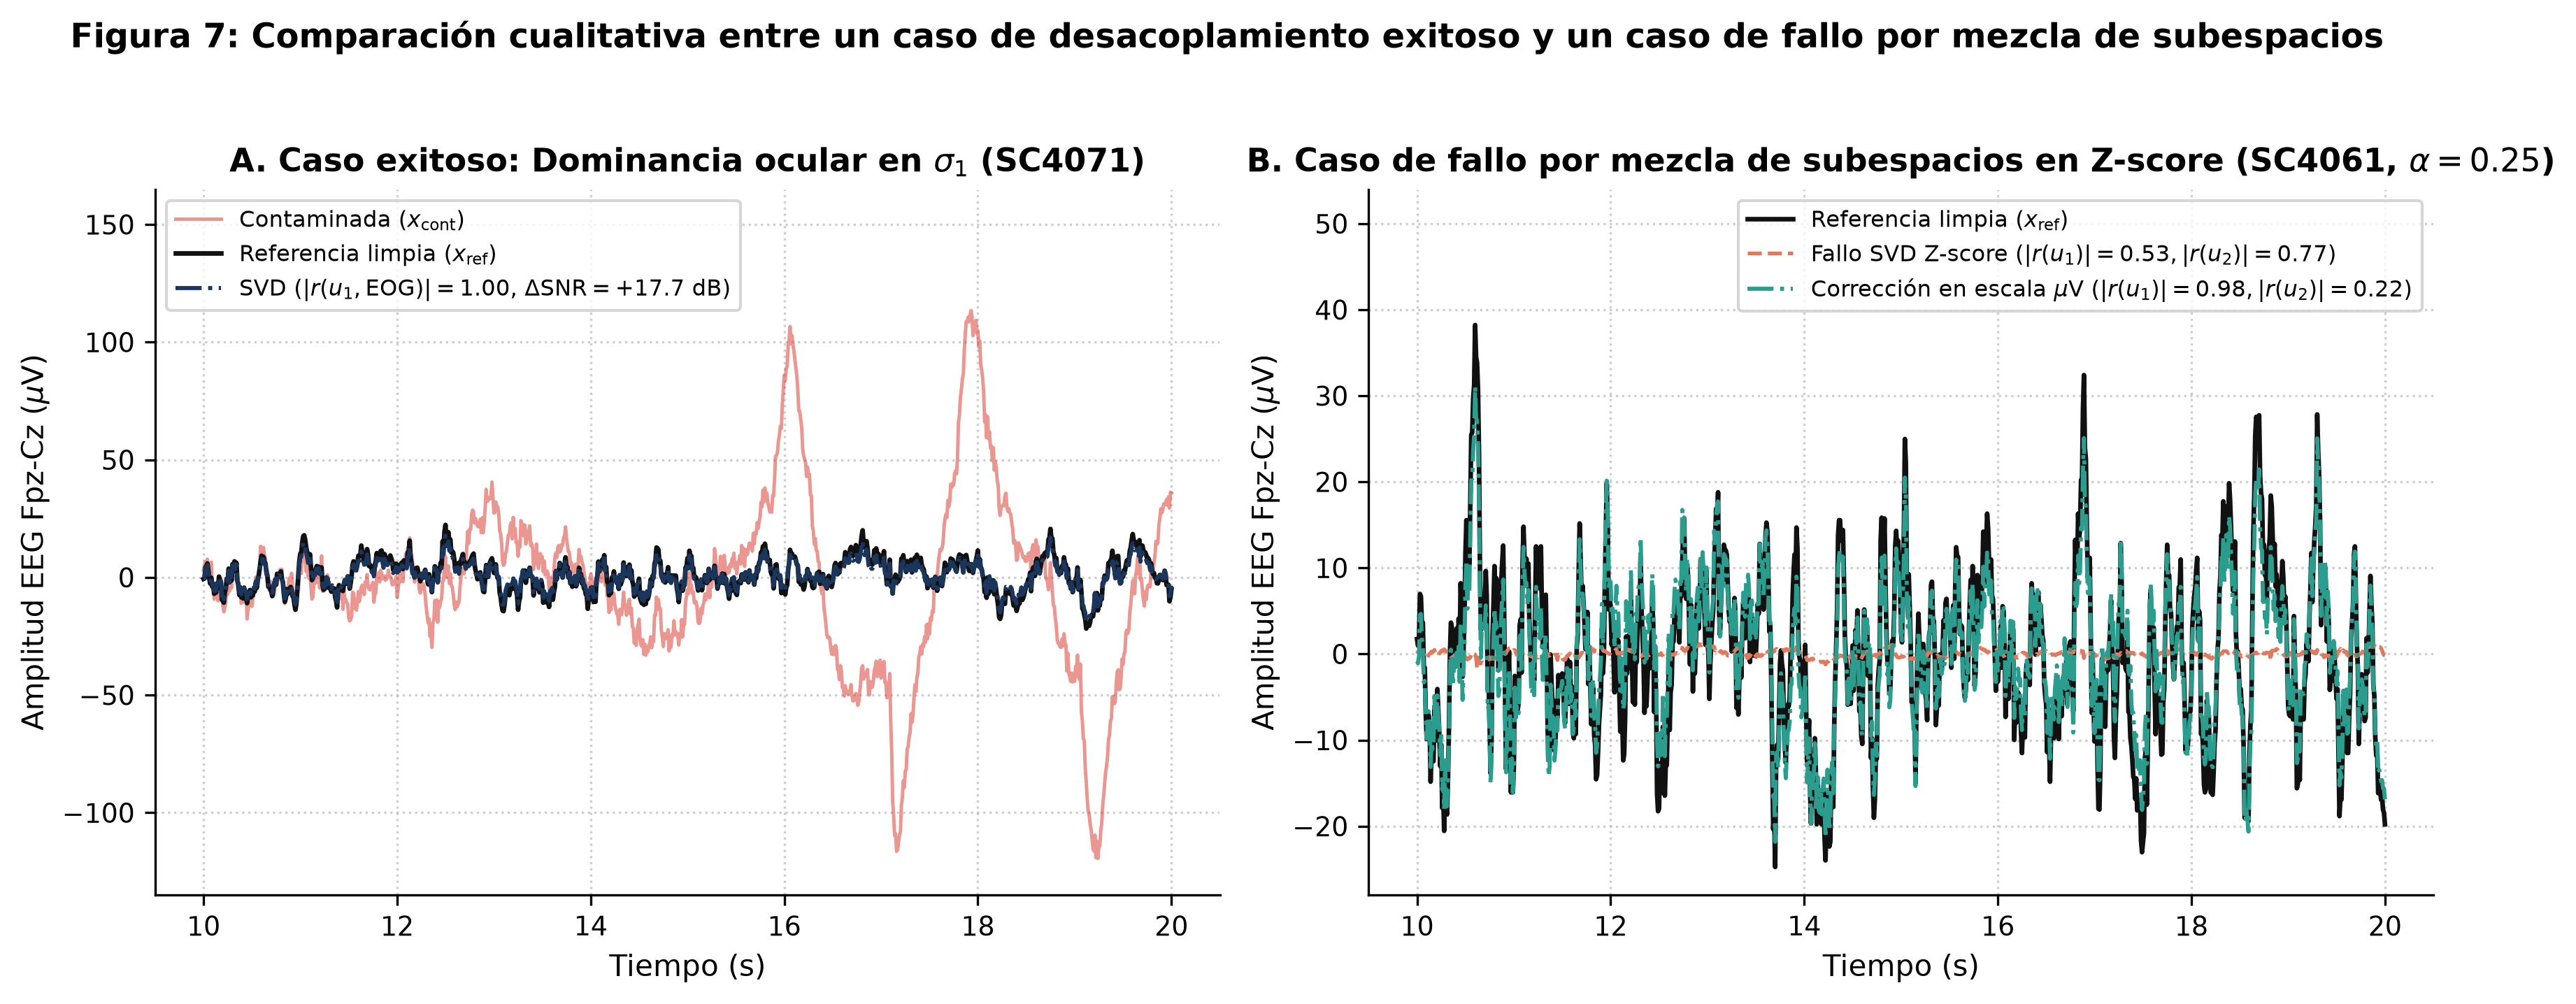
\includegraphics[width=\linewidth,height=4.85cm,keepaspectratio]{figures/fig7_exito_vs_fallo_svd.png}
      \end{tcolorbox}
    \end{column}

    \begin{column}{0.43\textwidth}
      \begin{tcolorbox}[redcard, title={\scriptsize\bfseries Explicaci\'on Intuitiva: ?`Por qu\'e falla Z-score en $\alpha=0.25$?}, colbacktitle=UDTerracotta!85!black, coltitle=white]
        \scriptsize
        \begin{enumerate}\setlength{\itemsep}{3pt}
          \item \textbf{En microvoltios ($\mu\text{V}$) el ojo es mucho m\'as grande:} El canal \texttt{EOG} ($\approx 39.7\,\mu\text{V}$) tiene casi \textbf{4 veces m\'as amplitud} que el \texttt{EEG} ($\approx 10.0\,\mu\text{V}$). Como la SVD ordena de mayor a menor energ\'ia, siempre pone al ojo primero ($\sigma_1 \gg \sigma_2$).
          \item \textbf{El Z-score encoge el EOG y agranda el EEG:} Al dividir cada canal por su desviaci\'on est\'andar, obligamos a los 3 canales a tener el mismo tama\~no (varianza $= 1$).
          \item \textbf{En contaminaci\'on baja ($\alpha=0.25$) se empatan las energ\'ias ($\sigma_1 \approx \sigma_2$):} Como ahora el artefacto ocular y el EEG pesan lo mismo, la SVD no logra separarlos y reparte el movimiento ocular entre el Modo 1 y el Modo 2. Al aplicar el umbral ($\tau^*=0.50$), borra 2 de los 3 modos en el $47.5\%$ de las \'epocas, da\~nando el EEG real.
        \end{enumerate}
      \end{tcolorbox}

      \vspace{0.06cm}

      \begin{tcolorbox}[tealcard]
        \tiny
        \textbf{Regla pr\'actica del proyecto:} Cuando se tiene un canal de referencia que mide directamente el artefacto de gran amplitud (EOG), \textbf{nunca se debe normalizar con Z-score}; se debe trabajar directamente en microvoltios ($\mu\text{V}$).
      \end{tcolorbox}
    \end{column}
  \end{columns}
\end{frame}

% ==============================================================================
% DIAPOSITIVA 13: DISCUSION, LIMITACIONES Y TRABAJO FUTURO
% ==============================================================================
\begin{frame}{La SVD supera el filtrado lineal sin entrenamiento, pero requiere ventanas adaptativas}
  \framesubtitle{Secci\'on 5: Discusi\'on cr\'itica, limitaciones metodol\'ogicas y trabajo futuro | Expositor: Cristian Aguilar}

  \begin{columns}[T,onlytextwidth]
    \begin{column}{0.32\textwidth}
      \begin{tcolorbox}[navycard, title={\scriptsize\bfseries 1. Discusi\'on frente al Estado del Arte}, colbacktitle=UDNavy, coltitle=white, equal height group=dlf]
        \scriptsize
        \begin{itemize}
          \item \textbf{Ventaja sobre Butterworth:} Confirma que cuando artefacto y se\~nal comparten la misma frecuencia ($0.5\text{--}4\text{ Hz}$), separar por componentes espaciales/temporales gana $+10.32\text{ dB}$ en $\alpha=0.50$.
          \item \textbf{Soluci\'on para pocos canales:} A diferencia de ICA que exige 16 o m\'as electrodos [4], [5], nuestra SVD funciona con los 3 canales b\'asicos de \textit{Sleep-EDF} [1].
          \item \textbf{Importancia de la amplitud f\'isica:} Confirma en la pr\'actica lo reportado por Lagerlund [8]: la SVD separa bien cuando el artefacto domina en amplitud ($\sigma_1 \gg \sigma_2$).
        \end{itemize}
      \end{tcolorbox}
    \end{column}

    \begin{column}{0.33\textwidth}
      \begin{tcolorbox}[redcard, title={\scriptsize\bfseries 2. Limitaciones del Estudio Actual}, colbacktitle=UDTerracotta!85!black, coltitle=white, equal height group=dlf]
        \scriptsize
        \begin{itemize}
          \item \textbf{Mezcla instant\'anea simple:} Nuestro experimento suma el EOG con un factor fijo $\alpha$ por \'epoca, sin simular retardos a trav\'es del cr\'aneo.
          \item \textbf{Ventana larga de $30\text{ s}$:} Calcula una sola SVD para todos los $30\text{ segundos}$, aunque los movimientos oculares ocurran solo en r\'afagas cortas.
          \item \textbf{Requiere el canal EOG conectado:} La regla de correlaci\'on $|r(u_i,\text{EOG})|\ge 0.50$ necesita que el electrodo ocular funcione correctamente.
        \end{itemize}
      \end{tcolorbox}
    \end{column}

    \begin{column}{0.32\textwidth}
      \begin{tcolorbox}[tealcard, title={\scriptsize\bfseries 3. Hoja de Ruta y Trabajo Futuro}, colbacktitle=UDTeal!85!black, coltitle=white, equal height group=dlf]
        \scriptsize
        \begin{itemize}
          \item \textbf{Ventanas cortas de $2\text{ a }5\text{ s}$:} Aplicar la SVD solo en los segundos exactos donde hay sacadas oculares, dejando intacto el resto de la \'epoca.
          \item \textbf{Detecci\'on sin canal EOG:} Identificar el modo ocular mirando qu\'e componente concentra demasiada energ\'ia lenta ($0.5\text{--}4\text{ Hz}$) [9] si el EOG se desconecta.
          \item \textbf{Prueba en clasificaci\'on de sue\~no:} Medir cu\'anto mejora la detecci\'on autom\'atica de sue\~no REM en los 197 registros de \textit{Sleep-EDF}.
        \end{itemize}
      \end{tcolorbox}
    \end{column}
  \end{columns}
\end{frame}

% ==============================================================================
% DIAPOSITIVA 14: CONCLUSIONES, REFERENCIAS Y ENLACE AL REPOSITORIO
% ==============================================================================
\begin{frame}{La SVD en escala f\'isica es una soluci\'on eficaz y reproducible para PSG de pocos canales}
  \framesubtitle{Secci\'on 5: Conclusiones principales, referencias IEEE y acceso al c\'odigo abierto | Expositores: Sergio Osorio y Nicolas Velasco}

  \begin{columns}[T,onlytextwidth]
    \begin{column}{0.53\textwidth}
      \begin{tcolorbox}[tealcard, title={\scriptsize\bfseries Conclusiones Verificadas de la Prueba de Concepto}, colbacktitle=UDTeal!85!black, coltitle=white]
        \scriptsize
        \begin{enumerate}\setlength{\itemsep}{2pt}
          \item \textbf{Se comprob\'o la hip\'otesis en sujetos nuevos:} En los 5 pacientes de Evaluaci\'on ($N_{\text{eval}}=183$ \'epocas REM), la SVD en microvoltios ($\mu\text{V}$) con $\tau^*=0.50$ alcanz\'o $\text{SNR}$ de $+18.37\text{ dB}$ ($\alpha=0.25$), $+11.39\text{ dB}$ ($\alpha=0.50$) y $+7.35\text{ dB}$ ($\alpha=0.80$), superando a la se\~nal cruda en $+13.9\text{ a }+14.9\text{ dB}$ y a Butterworth en $+9.1\text{ a }+14.5\text{ dB}$ con 95\% de confianza.
          \item \textbf{Se recuper\'o la banda delta sin deformar el EEG:} En $\alpha=0.50$, baj\'o el error de la onda (Frobenius) de $1.305$ a $0.257$ y redujo en un $66.8\%$ el error en banda delta ($0.5\text{--}4\text{ Hz}$) respecto a Butterworth.
          \item \textbf{La escala en microvoltios es indispensable:} Mantener las unidades reales ($\mu\text{V}$) permite que el ojo domine el Modo 1 ($\sigma_1 \gg \sigma_2$), evitando la mezcla de se\~nales que sufre el Z-score en baja contaminaci\'on.
        \end{enumerate}
      \end{tcolorbox}

      \vspace{0.05cm}

      \begin{tcolorbox}[navycard, title={\scriptsize\bfseries Reproducibilidad: Repositorio y Cuaderno Ejecutable}, colbacktitle=UDNavy, coltitle=white]
        \scriptsize
        \textbf{Enlace al repositorio / Notebook (\texttt{prueba\_concepto\_svd\_rem.ipynb}):}\\
        {\scriptsize\bfseries\color{UDNavy}\url{\RepoURL}}\\[0.03cm]
        {\tiny Descarga los registros reales de PhysioNet (\textit{Sleep-EDF v1.0.0}) y reproduce con semilla fija (\texttt{seed = 2026}) todas las tablas, m\'etricas y las 7 figuras.}
      \end{tcolorbox}
    \end{column}

    \begin{column}{0.45\textwidth}
      \begin{tcolorbox}[basecard, title={\scriptsize\bfseries Referencias Bibliogr\'aficas (Formato IEEE)}, colbacktitle=UDNavy, coltitle=white, top=3pt, bottom=3pt]
        \fontsize{5.1pt}{6.0pt}\selectfont\raggedright
        \textbf{[1]} B. Kemp \textit{et al.}, ``Analysis of a sleep-dependent neuronal feedback loop,'' \textit{IEEE Trans. Biomed. Eng.}, vol. 47, no. 9, pp. 1185--1194, 2000.\\[1.2pt]
        \textbf{[2]} G. Gratton \textit{et al.}, ``A new method for off-line removal of ocular artifact,'' \textit{Electroencephalogr. Clin. Neurophysiol.}, vol. 55, no. 4, pp. 468--484, 1983.\\[1.2pt]
        \textbf{[3]} P. Berg and M. Scherg, ``Dipole models of eye movements and blinks,'' \textit{Electroencephalogr. Clin. Neurophysiol.}, vol. 79, no. 1, pp. 36--44, 1991.\\[1.2pt]
        \textbf{[4]} S. Makeig \textit{et al.}, ``Independent component analysis of EEG data,'' \textit{Adv. Neural Inf. Process. Syst.}, vol. 8, pp. 145--151, 1995.\\[1.2pt]
        \textbf{[5]} R. N. Vig\'ario, ``Extraction of ocular artefacts from EEG using ICA,'' \textit{Electroencephalogr. Clin. Neurophysiol.}, vol. 103, no. 3, pp. 395--404, 1997.\\[1.2pt]
        \textbf{[6]} T.-P. Jung \textit{et al.}, ``Removing EEG artifacts by blind source separation,'' \textit{Psychophysiology}, vol. 37, no. 2, pp. 163--178, 2000.\\[1.2pt]
        \textbf{[7]} G. H. Golub and C. F. Van Loan, \textit{Matrix Computations}, 4th ed. Johns Hopkins Univ. Press, 2013.\\[1.2pt]
        \textbf{[8]} T. D. Lagerlund \textit{et al.}, ``Spatial filtering of multichannel EEG recordings through PCA by SVD,'' \textit{J. Clin. Neurophysiol.}, vol. 14, pp. 73--82, 1997.\\[1.2pt]
        \textbf{[9]} M. Gavish and D. L. Donoho, ``The optimal hard threshold for singular values is $4/\sqrt{3}$,'' \textit{IEEE Trans. Inf. Theory}, vol. 60, pp. 5040--5053, 2014.\\[1.2pt]
        \textbf{[10]} R. Ghosh \textit{et al.}, ``Automated ocular artifact removal in sleep EEG,'' \textit{Biomed. Signal Process. Control}, 2023.\\[1.2pt]
        \textbf{[11]} B. Salaman \textit{et al.}, ``SVD subspace filtering in biomedical signals,'' 2021.\\[1.2pt]
        \textbf{[12]} D. Grochala \textit{et al.}, ``Low-channel EEG artifact suppression,'' 2023.\\[1.2pt]
        \textbf{[13]} S. Phadikar \textit{et al.}, ``Hybrid wavelet-SVD ocular artifact removal in EEG,'' \textit{IEEE Access}, 2025.
      \end{tcolorbox}
    \end{column}
  \end{columns}
\end{frame}

\end{document}
